\documentclass[11pt, letterpaper]{arxiv}
\usepackage[all]{hypcap}
\usepackage[comma,numbers,sort,compress]{natbib}
\usepackage{hyperref}[citecolor=magenta]
\usepackage[capitalize,noabbrev]{cleveref}
\bibliographystyle{plainnat}

\hypersetup{
    colorlinks = true,
    citecolor = {magenta},
}

\usepackage{microtype}
\usepackage{graphicx}
\usepackage{subfigure}
\usepackage{booktabs} 

\usepackage{xcolor}
\usepackage{colortbl}
\usepackage{algorithm}
\usepackage{algpseudocode}
\usepackage{setspace}

% === Our Macros ===
\newcommand{\figurespace}{\vspace{-4mm}} 

\def\algorithmautorefname{Algorithm}
\renewcommand{\sectionautorefname}{\S}
\def\Snospace~{\S{}}
\renewcommand*\sectionautorefname{\Snospace}
\renewcommand{\subsectionautorefname}{\sectionautorefname}
\renewcommand{\subsubsectionautorefname}{\sectionautorefname}
\renewcommand*{\figureautorefname}{Fig.}
\renewcommand*{\tableautorefname}{Tab.}
\renewcommand*{\appendixautorefname}{App.}
\renewcommand*{\algorithmautorefname}{Alg.}
\newcommand{\etal}{\textit{et~al}.~\ }
\newcommand{\eg}{\textit{e.g.,}~}
\newcommand{\ie}{\textit{i.e.,}~}
\newcommand{\cf}{\textit{c.f.,}~}
\newcommand{\bg}{\texttt{BoxingGym}~}

% \newcommand{\alglabel}[1]{\label{alg:#1}}
% \newcommand{\algref}[1]{Alg~\ref{alg:#1}}
% \renewcommand*{\algorithmautorefname}{Alg.}
\newcommand\lt[2]{\mathcal{#1}_{\text{#2}}}
% \newcommand\st[2]{#1_{\text{#2}}}
% \newfloatcommand{capbtabbox}{table}[][\FBwidth]
\definecolor{coco1}{HTML}{D9E4EC}
\definecolor{coco2}{HTML}{B7CFDC}
\definecolor{coco3}{HTML}{6AABD2}
\definecolor{coco4}{HTML}{385E72}
\hypersetup{
    colorlinks=true,
    linkcolor=coco3,
    filecolor=coco4,      
    urlcolor=coco3,
    citecolor=coco3,
}

\newcommand{\ourmethod}{\texttt{GIANTS-4B}}
% Should we do GIANTS-Bench/GIANTS-BENCH to keep naming consistent
\newcommand{\ourbenchmark}{\textsc{GiantsBench}}
\newcommand{\benchmarknumdata}{$20k$}

\newcommand{\gemtwoflash}{\texttt{gemini-2.5-flash}}
\newcommand{\gemtwopro}{\texttt{gemini-2.5-pro}}
\newcommand{\gemthreepro}{\texttt{gemini-3-pro}}
\newcommand{\qwenfourb}{\texttt{Qwen3-4B}}
\newcommand{\qwenfourteenb}{\texttt{Qwen3-14B}}

\usepackage{float}



\usepackage{amsmath}
\usepackage{amssymb}
\usepackage{mathtools}
\usepackage{amsthm}

\usepackage{placeins}

\setlength\parindent{0pt}

\usepackage{fleqn, tabularx}

\usepackage{float}

\usepackage[most,skins,theorems]{tcolorbox}
\tcbset{
  aibox/.style={
    width=\linewidth,
    top=7pt,
    bottom=2pt,
    colback=blue!6!white,
    colframe=black,
    colbacktitle=black,
    enhanced,
    center,
    attach boxed title to top left={yshift=-0.1in,xshift=0.15in},
    boxed title style={boxrule=0pt,colframe=white,},
  }
}
\newtcolorbox{AIbox}[2][]{aibox,title=#2,#1}
\newcommand\myeq{\stackrel{\mathclap{\small\mbox{def}}}{=}}

\usepackage{wrapfig}
\definecolor{lightblue}{rgb}{0.22,0.45,0.70}
\usepackage{fleqn, tabularx}





\definecolor{rliableolive}{HTML}{BBCC33}
\definecolor{rliableblue}{HTML}{77AADD}
\definecolor{rliablered}{HTML}{EE8866}


\usepackage{crossreftools}
\pdfstringdefDisableCommands{%
    \let\Cref\crtCref
    \let\cref\crtcref
}
\newcommand{\creftitle}[1]{\crtcref{#1}}
\usepackage[suppress]{color-edits}
\newcommand{\tx}[1]{\txcomment{#1}}
\usepackage{dsfont}
\usepackage{nicefrac}
\newtcolorbox{analysisbox}[1][]{
    enhanced jigsaw,
    colback=white,
    colframe=blue!75!black,
    fonttitle=\bfseries,
    boxsep=5pt,
    left=5pt,
    right=5pt,
    top=5pt,
    bottom=5pt,
    title=#1,
}
\definecolor{editInitialResponse}{RGB}{255, 235, 156} 
\definecolor{editBacktrack}{RGB}{0, 0, 139}
\definecolor{editRevisedResponse}{RGB}{255, 182, 193}

\newcommand{\mistake}[1]{\sethlcolor{highlightmistake}\hl{#1}\sethlcolor{yellow}}
\newcommand{\correct}[1]{\sethlcolor{highlightcorrect}\hl{#1}\sethlcolor{yellow}}
\newcommand{\InitialResponse}[1]{\sethlcolor{editInitialResponse}\hl{#1}\sethlcolor{yellow}}
\newcommand{\Backtrack}[1]{\sethlcolor{editInitialResponse}\hl{#1}\sethlcolor{yellow}}
\newcommand{\RevisedResponse}[1]{\sethlcolor{editInitialResponse}\hl{#1}\sethlcolor{yellow}}
% \newcommand{\cmark}{\ding{51}}
% \newcommand{\xmark}{\ding{55}}
\usepackage{pifont}
\usepackage{soul}
\definecolor{highlightmistake}{RGB}{255, 179, 179} 
\definecolor{highlightcorrect}{RGB}{179, 255, 179} 
\newcommand{\rr}[1]{\textbf{\color{green}[RR: #1]}}

\usepackage[capitalize,noabbrev]{cleveref}

\theoremstyle{plain}
\newtheorem{theorem}{Theorem}[section]
\newtheorem{proposition}[theorem]{Proposition}
\newtheorem{lemma}[theorem]{Lemma}
\newtheorem{corollary}[theorem]{Corollary}
\theoremstyle{definition}
\newtheorem{definition}[theorem]{Definition}
\newtheorem{assumption}[theorem]{Assumption}
\theoremstyle{remark}
\newtheorem{remark}[theorem]{Remark}

\newcommand{\as}[1]{{\textcolor{red}{
{\textcolor{blue}{\textbf{AS}}}: #1}}}
\newcommand{\ak}[1]{{\textcolor{red}{
{\textcolor{blue}{\textbf{AK}}}: #1}}}
\newcommand{\yq}[1]{{\textcolor{red}{
{\textcolor{blue}{\textbf{YQ}}}: #1}}}
\newcommand{\my}[1]{{\textcolor{red}{
{\textcolor{blue}{\textbf{MY}}}: #1}}}
\newcommand{\bc}{\mathbf{c}}
\usepackage[textsize=tiny]{todonotes}
\usepackage{multirow}
\usepackage{enumitem}
\input{math_commands}

\newtcolorbox{promptbox}[2][]{  
listing only,
enhanced,
breakable,
colback=blue!6!white,
% colback=rliableolive!13!white,
colframe=black,
fontupper=\ttfamily,
title=#2,
#1}

\newcommand{\methodname}{{\texttt{GIANTS}}}

% \LARGE 
\title{\methodname{} : Generative Insight Anticipation from Scientific Literature}

\author[*1]{Joy He-Yueya}
\author[*1]{Anikait Singh}
\author[1]{Ge Gao}
\author[1]{Michael Y. Li}
\author[2]{Sherry Yang}
\author[1]{Chelsea Finn}
\author[1]{Emma Brunskill}
\author[1]{Noah D. Goodman}


\affil[1]{Stanford University}
\affil[2]{New York University}
\affil[*]{Equal contribution}

\correspondingauthor{heyueya@stanford.edu, anikait@stanford.edu. \newline \textbf{Project Website:} \textnormal{\url{https://cohenqu.github.io/rlad.github.io/}}}


\begin{document}

\maketitle

Scientific breakthroughs often emerge from synthesizing prior ideas into novel contributions. While language models (LMs) show promise in scientific discovery, their ability to emulate this targeted, evolutionary synthesis remains largely unexplored. We introduce insight anticipation, a novel literature-grounded generation task that moves beyond open-ended brainstorming by challenging models to predict a downstream paper's core contribution directly from the summaries of its foundational parent papers. To evaluate this capability, we develop \ourbenchmark{}, a large-scale benchmark comprising $17k$ tuples of parent and downstream papers across eight scientific domains. We assess performance using an LM judge to measure the similarity between generated and ground-truth insights, demonstrating a positive correlation with human expert evaluations. Finally, we present \ourmethod{}, an LM trained via reinforcement learning (RL) to optimize insight anticipation using these similarity scores as a proxy reward. Despite its smaller open-source architecture, \ourmethod{} significantly outperforms proprietary baselines, achieving a 34\% relative increase in similarity score compared to \gemthreepro{}. We release our code, dataset, and model to accelerate future research in automated scientific discovery.

\begin{flushright}
``If I have seen further than others, it is only because \\ I was standing on the shoulders of giants'' \\--- Sir Isaac Newton
\end{flushright}

\section{Introduction}
Language Models (LMs) are maturing into powerful tools for scientific discovery~\citep{karpathy2026autoresearch}. Early milestones are striking, from virtual LM teams designing SARS-CoV-2 nanobody binders~\citep{swanson2025virtual} to models proposing NLP research directions that human experts rate as genuinely novel~\citep{si2024can}. However, these successes rely heavily on prompting existing frontier models that are extensively pre-trained on massive corpora of text. In contrast, human scientists achieve breakthroughs through a far more efficient process: by synthesizing profound insights from sparse and disparate sources. Emulating this human-like capability of conjecturing is not just a theoretical ideal; it is a practical necessity as LMs struggle to reliably generate ideas of true impact and value~\citep{si2025ideation}, often due to the lack of diversity and feasibility~\citep{wadhwa2026createtestingllmsassociative}. 

To bridge this gap, we propose a new paradigm: \emph{insight anticipation}. Rather than focusing on broad data assimilation, this setting tasks models with predicting the natural evolutionary trajectory of specific, existing research. This framing adopts the classical view of scientific progress as `\emph{standing on the shoulders of giants,}' where new contributions emerge by building incrementally upon prior foundations. Under this view, a paper’s value is defined by its relative advancement over the works it builds upon. Consequently, the challenge of automated discovery decomposes into two distinct subproblems: (1) \textit{parent selection}, or identifying which prior works to build upon, and (2) \textit{insight generation}, or synthesizing those works into a novel contribution.

This motivates a fundamental feasibility question: if provided with the relevant lineage of background papers, can a model effectively predict the next logical leap? In this work, we focus exclusively on the generation phase. By assuming the "parent" papers are provided by an oracle literature selection criterion, we test a model's capacity to transform these foundations into a downstream paper’s primary insight. While identifying optimal parent papers remains a complex challenge of scientific attribution, isolating the generation phase allows us to rigorously evaluate the creative potential of targeted synthesis, leaving retrieval strategies for future work.

\begin{figure}[t]
    \centering
    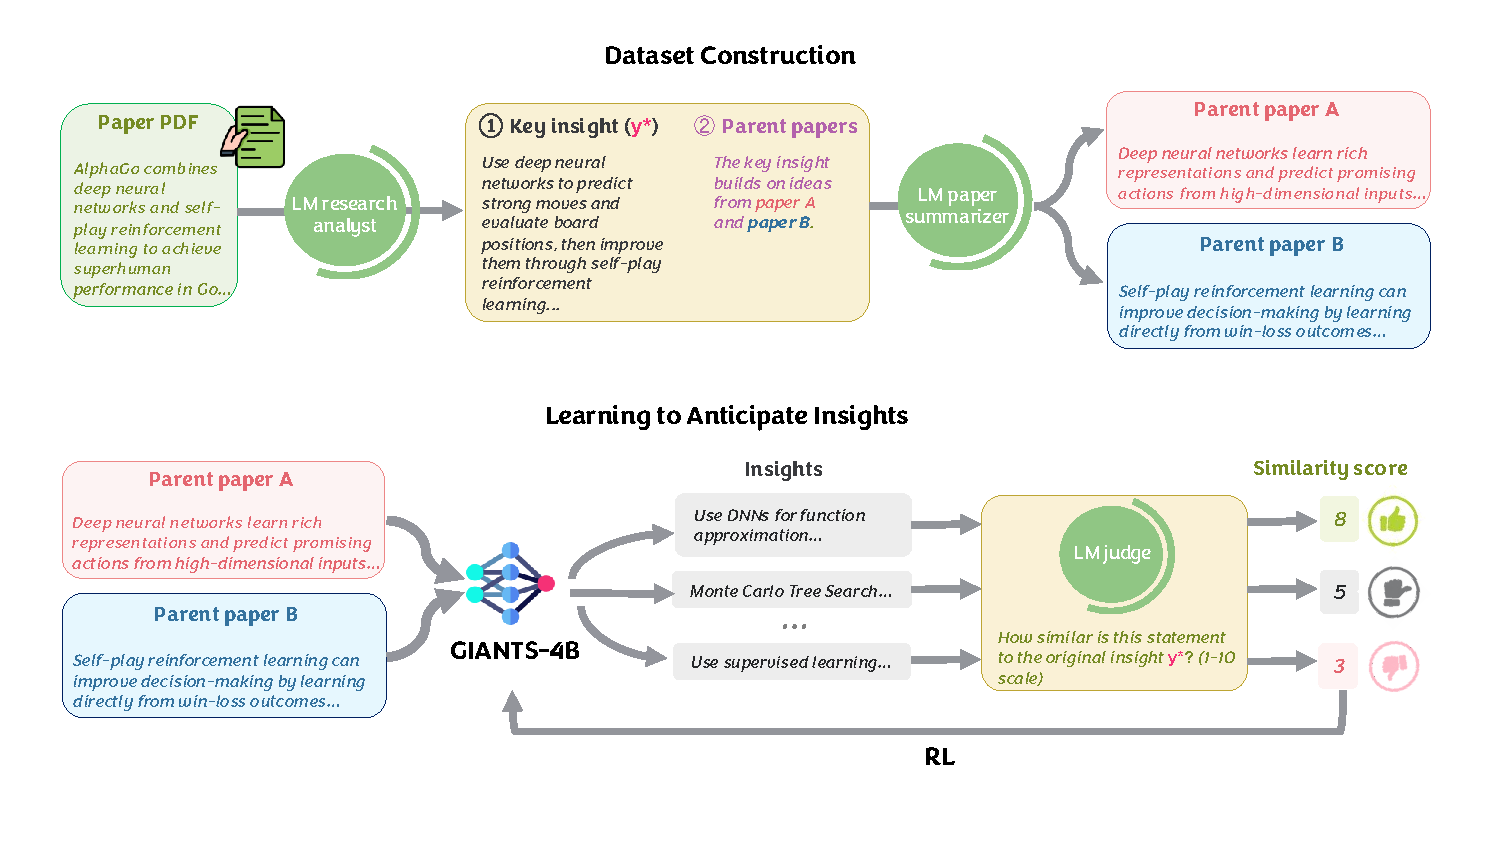
\includegraphics[width=\linewidth]{figs/giants_fig1.pdf}
    \vspace{-3mm}
    \caption{\footnotesize \textbf{Overview of \ourbenchmark{} and \ourmethod{}.} \textit{(top)} For dataset construction, we use an LM as a research analyst to process each paper PDF to identify two parent papers whose ideas are synergistically combined to produce the paper's key insight, which is extracted as the ground-truth target $y^*$. A second LM summarizes each parent paper. \textit{(bottom)} Given the two parent summaries, the model generates candidate insights, which an LM judge scores by similarity to $y^*$ on a 1–10 scale. These scores serve as a proxy reward for RL training, teaching the model to anticipate insights that more closely match real downstream papers.}
    \label{fig:giants_fig1}
    \vspace{-3mm}
\end{figure}

To evaluate insight anticipation models, we develop \ourbenchmark{}, a large-scale benchmark designed to evaluate the ability of models to synthesize two prior papers and derive the core insight of a downstream paper that builds on them (Figure~\ref{fig:giants_fig1}, top). Unlike previous benchmarks that evaluate the ability of models to answer literature synthesis questions by identifying relevant papers and generating long-form responses with citations \citep{asai2026synthesizing}, \ourbenchmark{} assesses whether a model can combine two parent papers synergistically to derive insights that lead to a subsequent paper. \ourbenchmark{} comprises $17k$ input pairs of parent paper summaries and their corresponding downstream research insights, drawn from Computer Science, Economics, Electrical Engineering, Mathematics, Physics, Quantitative Biology, Quantitative Finance, and Statistics. We also introduce an automatic evaluation method that uses an LM judge to give a \textbf{similarity score} comparing the model-generated insight to the ground-truth insight. We conducted expert evaluations of the LM judge and found that LM scores and human scores are positively correlated (Spearman's $\rho = 0.761$, $p < 0.001$).

Furthermore, we introduce \ourmethod{}, a language model trained to generate the core insight of a future scientific paper given a set of prior papers via reinforcement learning (RL). By fine-tuning with GRPO \citep{shao2024deepseekmath} to maximize the similarity scores on the research insights, the model learns to reason about connections between the input papers and generate insights that are more similar to those from real downstream papers (Figure~\ref{fig:giants_fig1}, bottom). This outperforms simply distilling the expert insight (even with reasoning traces).

We evaluate proprietary and open LMs (e.g., \gemtwopro{}, \gemthreepro{}, \qwenfourb{})
on \ourbenchmark{}. \qwenfourb{} performs similarly as \gemtwopro{} and \gemthreepro{}, despite being a smaller open model, which shows that LMs are not simply getting better at insight anticipation via scaling. In contrast, our \ourmethod{}, which uses RL with similarity scores from the LM judge as a proxy reward, significantly improves insight anticipation. 

We summarize our main contributions as follows:
\begin{itemize}
    \item \textbf{Novel paradigm for automated discovery}: We introduce the task of \emph{insight anticipation}, which isolates the creative synthesis phase of scientific progress by evaluating how effective a model is at predicting a downstream paper's core insight conditioned on foundational parent papers.
    \item \textbf{\ourbenchmark{} and evaluation metric}: We source a dataset of 17k tuples of parent and downstream papers from arXiv across eight domains and have an LM-based auto-evaluator to score the similarity between generated and ground-truth insights.
    \item \textbf{\ourmethod{}}: We present a novel approach for training a model for insight anticipation based on semantic similarity and RL, outperforming a range of proprietary and open LMs such as \gemthreepro{}.
\end{itemize}


% \footnote{\href{https://docs.cloud.google.com/vertex-ai/generative-ai/docs/models/gemini/2-5-pro}{https://docs.cloud.google.com/vertex-ai/generative-ai/docs/models/gemini/2-5-pro}}
% \footnote{\href{https://docs.cloud.google.com/vertex-ai/generative-ai/docs/models/gemini/3-pro}{https://docs.cloud.google.com/vertex-ai/generative-ai/docs/models/gemini/3-pro}}
% \footnote{\href{https://huggingface.co/Qwen/Qwen3-4B}{https://huggingface.co/Qwen/Qwen3-4B}}
% This formulation serves as a stepping stone toward the broader goal of predicting future research directions.






\section{Defining and Instantiating a Benchmark for Insight Anticipation}
\label{sec:dataset_construction}

\paragraph{Task Definition.} We introduce the setting of insight anticipation: given an input context with two paper summaries $x = (x_A, x_B)$ where $x_A$ is a summary of paper $A$, and $x_B$ is a summary of paper $B$, the goal is to generate the key insight of a downstream paper that builds on $A$ and $B$. We denote this ground truth downstream insight statement as $y^*$. $y^*$ is an oracle insight that emerges only when both papers are considered together. This task requires the model to consider how $A$ and $B$ might jointly influence a downstream paper and generate a research insight/idea $\hat{y}$ that is semantically similar to $y^*$. This setup intentionally restricts the number of parents to two (as more papers lead to context management constraints for training and inference), making the task a conservative lower bound on the full problem. We do not address parent discovery, focusing instead on whether meaningful insight synthesis is possible given fixed inputs. Figure~\ref{fig:insight_generation_prompt} shows the insight generation prompt we use for training or evaluating all models. 


\paragraph{Dataset Construction.}
We create a dataset $\{((x_A, x_B)_i, y^*_i)\}_{i=1}^N$ as follows. We collect $17{,}839$ papers from arXiv that are published between May 23rd, 2007, and January 23rd, 2026, according to their latest update date on arXiv. Since arXiv is not peer reviewed, the raw corpus may contain noisy or non-substantive documents. To mitigate this, we retain only papers with at least two citations.\footnote{We use citation counts from Semantic Scholar as a proxy for paper quality.} We download these papers as a PDF. For each paper, we prompt \gemtwoflash{}
% \footnote{\href{https://docs.cloud.google.com/vertex-ai/generative-ai/docs/models/gemini/2-5-flash}{https://docs.cloud.google.com/vertex-ai/generative-ai/docs/models/gemini/2-5-flash}}
to identify two prior papers that this paper explicitly cites and builds upon by combining their ideas in a synergistic way. We also ask \gemtwoflash{} to explain the synergy (see the full prompt in Figure~\ref{fig:upstream_citation_prompt}). We then download the two parent papers as a PDF and use their content as input context $x$. Ideally, we would like to take the full paper content as input to the model and ask it to generate a downstream insight. However, given the context-length limitations of existing LMs as well as the high inference cost, we instead opt to prompt \gemtwoflash{} to summarize the paper. We then use paper summaries as the input. 
We use the following prompt to summarize each paper into key insights and contributions: ``\textit{Summarize the document, clearly describing the method used and highlighting the key insights or findings. Provide sufficient detail so that the approach and main contributions are fully understood.}'' 
For $y^*$, we use the synergy explanation that is part of the output to the parent-identification prompt in Figure~\ref{fig:upstream_citation_prompt}). 
% This next sentence is a bit unclear in terms of what explanation you are referring to. Could be useful to reword.
We cannot use the raw explanation because it refers to a future downstream paper and talks about the insight in the context of the two parent papers. Instead, we would like the model to generate a standalone insight statement directly from the two parent papers alone. Therefore, we prompt \gemthreepro{} to rewrite the insight and explanation without reference to the downstream paper (see prompt in Appendix~\ref{appendix:rewriting_insight_prompt}). After constructing all $(x,y^*)$ pairs, for each unique pair of parent papers $x=(x_A, x_B)$, we keep the insight $y^*$ from the most cited downstream paper in order to prioritize generating more impactful insights.

% TODO: Figure out location for this
\begin{wrapfigure}{r}{0.4\textwidth}
    \centering
    \vspace{-8mm}
    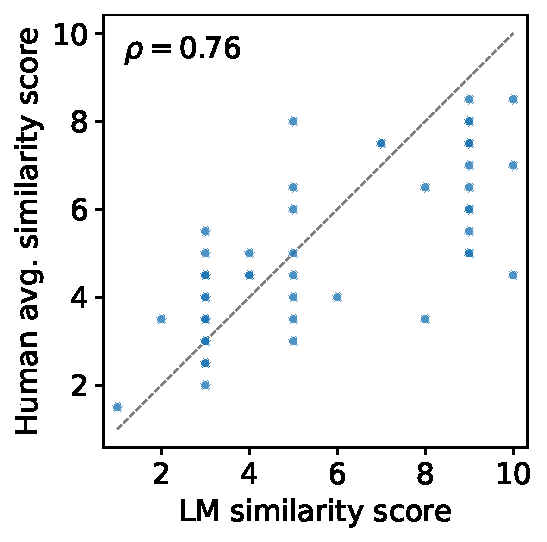
\includegraphics[width=0.9\linewidth]{figs/lm_vs_human_scatterplot.pdf}
    \caption{\footnotesize \textbf{Human experts align with LM judge.} LM similarity scores are positively correlated with human similarity scores (Spearman $\rho = 0.761$, $p < 0.001$, $n = 60$).}
    \label{fig:lm_vs_human_scatterplot}
    \vspace{-0.5cm}
\end{wrapfigure}
\paragraph{Temporal Hold-Out Evaluation.}
To more rigorously assess generalization, we conduct all evaluations on a \emph{future held-out test set} consisting of downstream papers published after the training cutoff date. We split the dataset by the publication date of the downstream paper in each $(x, y^*)$ pair. Papers published before July 1st, 2023 are used for training. To study the ability of models to generalize to new domains, we restrict the training set to papers tagged with cs.CL (Computation and Language), yielding $N=10{,}335$ training examples. For evaluation, we consider papers published after July 1, 2023 and randomly sample up to $600$ papers from each domain (see the category taxonomy in Appendix~\ref{appendix:domain_mapping}), resulting in a test set of $7{,}504$ papers. No papers from this test set are seen during training, though some of them may share at most 1 parent paper with the papers in the training set. We also conduct evaluations on a subset of the test set that does not have any overlapping parents with those in the training set. We call the subset \textbf{Test-unseen-parents} ($N=5{,}294$).

\paragraph{Evaluation Metric.}
For each generation, we prompt an LM judge to give a \textbf{similarity score} ranging from 1 to 10 (higher is better) comparing the model-generated insight to the ground-truth insight $y^*$. We use \gemthreepro{} as the judge model (see Figure~\ref{fig:similarity_judge_prompt} for the prompt). To assess the reliability of the LM-based evaluation, we conduct a human evaluation study on $30$ pairs of insights generated by \qwenfourb{} and \ourmethod{} ($n = 60$). Two human annotators, who are PhD students in Computer Science, independently rate the similarity between model-generated insights and ground-truth insights using the same rating scale as the LM judge. The LM’s scores show a statistically significant positive correlation with the average scores across human annotators (Figure~\ref{fig:lm_vs_human_scatterplot}). In particular, we observe a Spearman rank correlation of $\rho = 0.761$ ($p < 0.001$). More details can be found in Appendix~\ref{app:human_eval}.

\begin{AIbox}{Takeaways of Insight Anticipation Instantiation}
We introduce the \emph{insight anticipation} task, which challenges models to generate a future research insight by synthesizing the summaries of two parent papers. To evaluate this, we construct a dataset of over 17k arXiv paper triplets with LLM-extracted ground truths, utilizing a strict temporal/cross-domain hold-out split and a human-validated LLM judge for robust scoring.
\end{AIbox}

% This temporal split reflects a realistic forecasting setting: models are asked to predict insights for papers that did not yet exist at training time. As a result, performance cannot be attributed to memorization or leakage from the training corpus.

% We report all quantitative results, including LM-based similarity scores and human validation statistics, exclusively on this future held-out set. This design ensures that our evaluation measures the model’s ability to extrapolate from prior literature rather than reconstructing known outcomes.

% This produces a supervised learning signal linking prior work to downstream scientific contributions.



% We do this dataset collection effort
% Be careful about years (hold out)
% Doing it on whole papers would be cool but is a very long context task and it’s hard
% We first summarize the parent papers into key insights and we work at the level of key insights

\section{Training an Insight Anticipator}
We explore two primary training paradigms to optimize \ourmethod{} for insight anticipation: (1) distillation via supervised fine-tuning (SFT), leveraging ground-truth insights and rationalization from target papers, and (2) reinforcement learning (RL) for insight anticipation via similarity optimization. Across all experiments, we adopt \qwenfourb{} as our base model. Next, we will detail the specific formulations of these training methodologies.

\subsection{Ground Truth Insight Distillation via Supervised Fine-Tuning (SFT)}
The objective of our SFT pipeline is to adapt the base language model to synthesize a cohesive, derivative insight given the textual context of two source papers. We investigate two distinct SFT strategies to achieve this. In our standard SFT approach, the model is directly fine-tuned to map the input context (summaries of parent papers), $x$, to the target ground-truth insight, $y^*$ (derived from the target paper). This process optimizes the standard negative log-likelihood loss for autoregressive LMs over the paired examples $(x, y^*)$.

To bridge the logical gap between the source papers and the final insight, we also evaluate an SFT strategy enhanced with chain-of-thought reasoning~\citep{wei2023chainofthoughtpromptingelicitsreasoning}, which we denote as \emph{SFT-think}. In this setup, we introduce an intermediate synthetic rationalization step, $z$. To generate a supervision target, we prompt a high-capacity teacher model (\gemthreepro{}) to generate a detailed chain-of-thought that logically deduces the ground-truth insight conditioned on the parent paper summaries (as detailed in Section~\ref{sec:dataset_construction}). The base model is then trained to sequentially predict the rationale followed by the final insight, utilizing the augmented tuples $(x, z, y^*)$. This approach explicitly encourages the model to internalize the step-by-step inferential process rather than merely memorizing the final output mapping. This follows distillation approaches in reasoning as seen in works such as OpenThoughts~\citep{guha2025openthoughtsdatarecipesreasoning} and s1~\citep{muennighoff2025s1simpletesttimescaling}.

\begin{figure}[t]
    \centering
    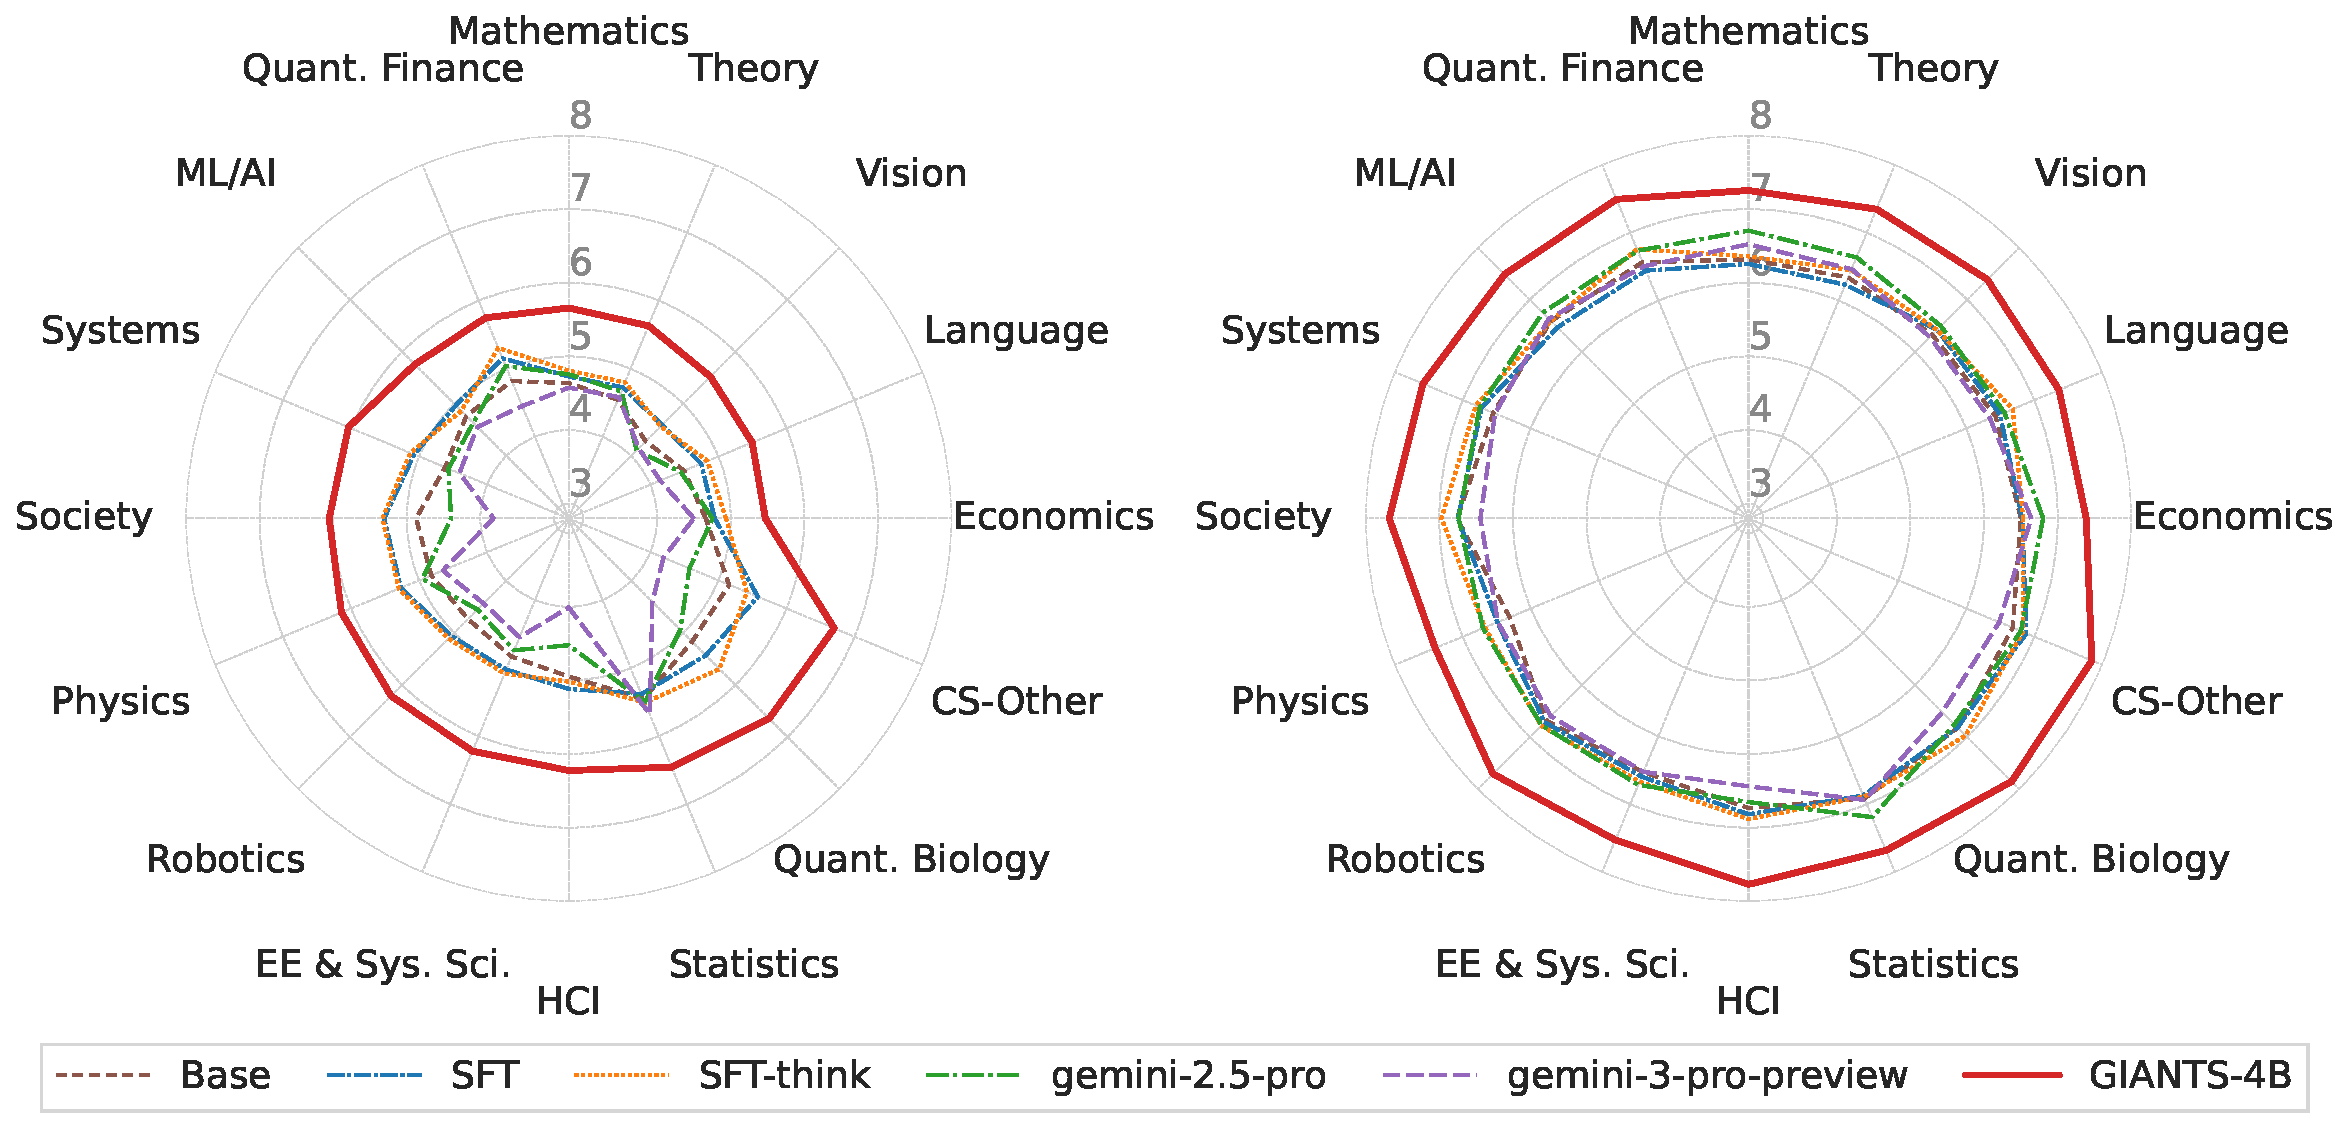
\includegraphics[width=0.9\linewidth]{figs/all_domain_radar_comparison_gemini-3-pro-preview_vs_Qwen3-14B.pdf}
    \vspace{-3mm}
    \caption{\footnotesize \textbf{Insight anticipation for arXiv domains.} \ourmethod{} has a higher similarity score to the target insight, outperforming SFT, SFT-Think, and the base model (\qwenfourb{}) for two different judge models.  The relative ordering of similarity scores for each domain, judged by \gemthreepro{} \textit{(left)} matches the ordering of similarity scores judged by \qwenfourteenb{} \textit{(right)}.}
    \label{fig:all_domain_radar_comparison_gemini-3-pro-preview_vs_Qwen3-14B}
\end{figure}

\begin{figure}[t]
    \centering
    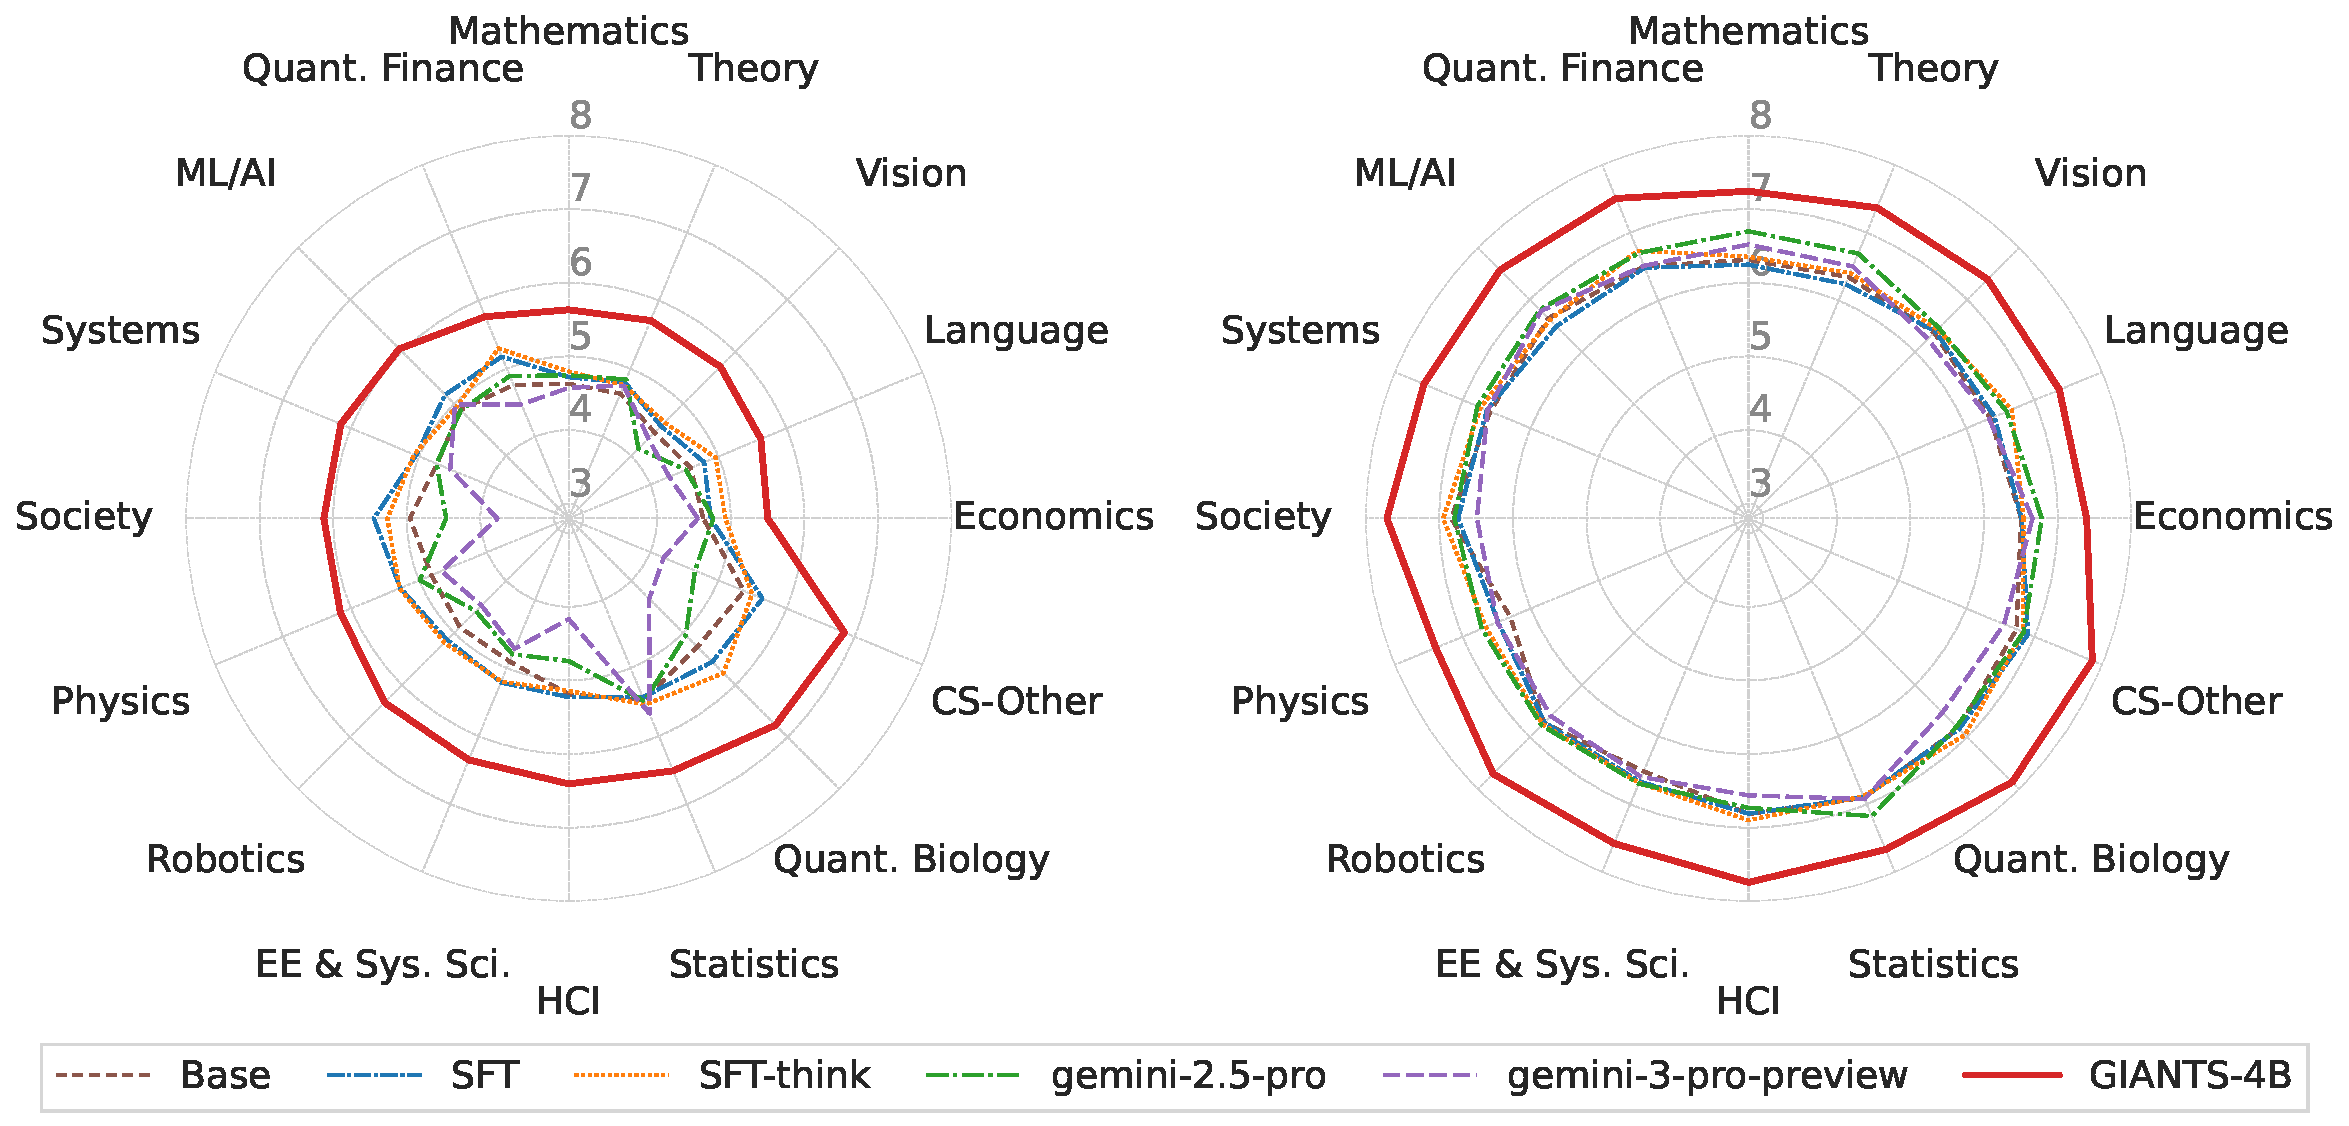
\includegraphics[width=0.9\linewidth]{figs/all_domain_radar_comparison_gemini-3-pro-preview_vs_Qwen3-14B_unseen_parents.pdf}
    \vspace{-3mm}
    \caption{\footnotesize \textbf{Similarity scores on \emph{Test-unseen-parents}}. This is the subset of \ourbenchmark{} test set with only unseen parent papers, where \ourmethod{} outperforms the base model and SFT both when judged by \gemthreepro{} \textit{(left)} and \qwenfourteenb{} \textit{(right)}.}
    \label{fig:all_domain_radar_comparison_gemini-3-pro-preview_vs_Qwen3-14B_unseen_parents}
    \vspace{-3mm}
\end{figure}

% (1) directly finetuning on $(x, y^*)$, and (2) finetuning on $(x, z, y^*)$ where the model generates chain-of-thought reasoning $z$ before the insight statement $y^*$. In the training data, $z$ is the generated by \qwenfourteenb{} when rewriting the insight (see Section~\ref{sec:dataset_construction}).

% The LM as Judge thing seems a bit weaker -> Changed to Insight Similarity
\subsection{Reinforcement Learning for Insight Anticipation via Similarity Optimization}
So far, we have explored distilling insights via supervised fine-tuning (SFT). However, in complex tasks such as scientific discovery, the target paper's insights can be difficult to clone directly. This difficulty often arises when the target insight has low likelihood under the policy, or when the model lacks the capacity to adequately capture the distribution of the parent insight. Can we instead consider an alternative approach that relies on reinforcement learning to recover the performance of the target paper's insights?

To address this, we employ an alternative approach: using the target paper's insights $y^{*}$ to define a proxy reward via a semantic similarity metric. Formally, given an insight from the target paper $y^{*}$, we define the proxy reward for a predicted insight $\hat{y}$ as: 
\begin{align}
    r_{\text{sim}}(\hat{y}) = \textit{similarity}(\hat{y}, y^{*})
\end{align}
where $\textit{similarity}$ measures the semantic equivalence between the generated insight and target insights measured using an LM-as-a-Judge~\citep{gu2025surveyllmasajudge}, matching the evaluation criterion in Section~\ref{sec:dataset_construction}. Furthermore, for further robustness and reducing order bias, we supply the LM with insights twice ($\hat{y}$ first, and $y^{*}$ first), taking the average over the individual similarity scores to compute the proxy reward. 
This proxy reward is then optimized via RL to recover the behavior of the ground-truth insight of the child paper conditioned on the two prespecified parent papers.

More concretely, we train \ourmethod{} using Group Relative Policy Optimization (GRPO) \citep{shao2024deepseekmath}, utilizing an LM as a proxy reward function. Specifically, for each input context $x$, we sample a group of $G=8$ candidate insights from the active policy. An LM judge evaluates these candidates and assigns scalar rewards based on a predefined similarity score metric (illustrated in Figure~\ref{fig:giants_fig1}, bottom). GRPO is well-suited for this setup because it optimizes the policy relative to the sampled group, thereby removing the need to train and maintain a separate, memory-intensive value function model.

Crucially, to mitigate the risk of reward hacking and ensure a rigorous evaluation, we enforce a strict separation between the training and testing judges. We deploy \gemtwoflash{} as the active reward model during GRPO training, while reserving the independent \gemthreepro{} model exclusively for the final evaluation phase. This decoupling guarantees a more objective, unbiased assessment of the model's true generalization capabilities. We additionally evaluate with other LM judges (e.g., \qwenfourteenb{}) to showcase robustness across model families.
% \footnote{\href{https://huggingface.co/Qwen/Qwen3-14B}{https://huggingface.co/Qwen/Qwen3-14B}}

\begin{AIbox}{Takeaways of Training an Insight Anticipator}
We optimize our insight anticipator using reinforcement learning to maximize semantic similarity to target insights. We strictly separate the LLM judges used for training and final evaluation.
\end{AIbox}


% Old Text
\iffalse

 We explore two training approaches: (1) Supervised fine-tuning on ground-truth insights, and (2) Reinforcement learning with an LLM as a judge. For all experiments we use \qwenfourb{} as the model being trained.


A base LM is fine-tuned to generate the downstream insight given two parent papers using standard supervised objectives. We compare two SFT approaches: \begin{itemize} \vspace{-10pt} \item \textbf{SFT}: We finetune the model on $(x, y^*)$. \vspace{-6pt} \item \textbf{SFT-think}: We generate synthetic chain-of-thought reasoning $z$ that leads to the ground-truth insight by prompting \gemthreepro{} (see Section~\ref{sec:dataset_construction}). Then, we conduct SFT on these synthetic thoughts with the ground-truth insights (i.e., $(x, z, y^*)$). \end{itemize}

We train \ourmethod{} using Group Relative Policy Optimization (GRPO; \citet{shao2024deepseekmath}) with rewards provided by an LM judge. Note that we use \gemtwoflash{} as the LM judge in training, different from the judge \gemtwopro{} in testing, to ensure a more reliable and unbiased evaluation. For each context, we sample $G=8$ candidate responses and compute rewards based on the similarity score evaluated by the LM judge (Figure~\ref{fig:giants_fig1}, right).
 
\fi

% \subsection{Frontier Model Baselines}
% We evaluate large frontier language models using zero-shot prompting as a reference baseline.

% TODO: try other model families


% \paragraph{LM-Based Similarity Judgment.}

% Our primary evaluation signal is based on a language model acting as a judge. For each generated insight, the judge assigns a similarity-based score comparing the model-generated insight to the ground-truth insight of the downstream paper.

% This similarity score is used both: (1) As a reward signal during reinforcement learning fine-tuning, and (2) As the main quantitative metric for comparing model variants at evaluation time.

% This approach enables scalable evaluation over a large corpus of papers, but raises the question of how well the LM-based judgments align with human evaluations.



% \subsection{Implications for Evaluation}

% Taken together, these results suggest that LM-based judgment provides a noisy but informative evaluation signal. While absolute score calibration remains imperfect, the strong correlation with human consensus supports its use for:
% \begin{itemize}
%     \item Model comparison
%     \item Reinforcement learning optimization
%     \item Large-scale evaluation where human annotation is infeasible
% \end{itemize}

% We therefore treat LM judgment as an approximate but practically useful proxy for human evaluation, and report human validation results to contextualize its limitations.






\section{Experimental Evaluation on \ourbenchmark{}}

% \begin{table}[t]
% \begin{center}
% \begin{tabular}{lcc}
% \toprule
% \multicolumn{1}{c}{\bf Model} 
% & \multicolumn{1}{c}{\bf Test set ($N=7k$)} 
% & \multicolumn{1}{c}{\bf Test-unseen-parents ($N=3k$)} \\
% \midrule
% Base (\qwenfourb)        & $6.6$   & $6.698$ \\
% SFT (\qwenfourb)         & $6.456$ & $6.468$ \\
% SFT-think (\qwenfourb)   & $6.674$ & $6.744$ \\
% \gemtwopro{}               & $6.903$ & $7.038$ \\   
% \gemthreepro{}             & $6.866$ & $7.059$ \\ 
% \ourmethod{} (\qwenfourb{} after RL)          & $\textbf{8.455}$  & $\textbf{8.542}$ \\
% \midrule
% \textit{Relative improvement} 
% & $\mathbf{22.5\%}$ 
% & $\mathbf{21\%}$ \\
% \bottomrule
% \end{tabular}
% \end{center}
% \caption{Average similarity scores on \ourbenchmark{}. \ourmethod{} outperforms the base model and other frontier models. \textbf{Test-unseen-parents} indicates the subset of test set with only unseen parent papers.}
% \label{table:main_results}
% \end{table}

% \begin{table}[t]
% \centering
% \resizebox{\textwidth}{!}{%
% \begin{tabular}{lccccccccccccccccc}
% \toprule
% \textbf{Model} & \textbf{Vision} & \textbf{Mathematics} & \textbf{Economics} & \textbf{Language} & \textbf{Theory} & \textbf{Systems} & \textbf{ML/AI} & \textbf{Physics} & \textbf{Robotics} & \textbf{EE \& Sys.} & \textbf{Society} & \textbf{HCI} & \textbf{Quant. Fin.} & \textbf{Statistics} & \textbf{CS-Other} & \textbf{Quant. Bio.} & \textbf{Overall} \\
% \midrule
% Base (\qwenfourb) & $4.28_{{\pm0.10}}$ & $4.64_{{\pm0.11}}$ & $4.66_{{\pm0.21}}$ & $4.50_{{\pm0.10}}$ & $4.54_{{\pm0.10}}$ & $4.62_{{\pm0.11}}$ & $4.77_{{\pm0.11}}$ & $4.82_{{\pm0.11}}$ & $4.74_{{\pm0.11}}$ & $4.83_{{\pm0.11}}$ & $4.87_{{\pm0.14}}$ & $4.95_{{\pm0.12}}$ & $4.82_{{\pm0.25}}$ & $5.45_{{\pm0.16}}$ & $5.16_{{\pm0.16}}$ & $5.17_{{\pm0.17}}$ & $4.75_{{\pm0.03}}$ \\
% SFT (\qwenfourb) & $4.59_{{\pm0.10}}$ & $4.73_{{\pm0.10}}$ & $4.78_{{\pm0.20}}$ & $4.75_{{\pm0.10}}$ & $4.72_{{\pm0.10}}$ & $5.07_{{\pm0.11}}$ & $4.97_{{\pm0.11}}$ & $5.27_{{\pm0.11}}$ & $5.06_{{\pm0.11}}$ & $5.02_{{\pm0.11}}$ & $5.31_{{\pm0.14}}$ & $5.12_{{\pm0.11}}$ & $5.15_{{\pm0.23}}$ & $5.38_{{\pm0.15}}$ & $5.58_{{\pm0.16}}$ & $5.43_{{\pm0.17}}$ & $5.01_{{\pm0.03}}$ \\
% SFT-think (\qwenfourb) & $4.57_{{\pm0.10}}$ & $4.81_{{\pm0.10}}$ & $4.94_{{\pm0.21}}$ & $4.84_{{\pm0.11}}$ & $4.80_{{\pm0.11}}$ & $5.13_{{\pm0.11}}$ & $4.87_{{\pm0.11}}$ & $5.30_{{\pm0.11}}$ & $5.11_{{\pm0.11}}$ & $5.08_{{\pm0.11}}$ & $5.33_{{\pm0.15}}$ & $5.02_{{\pm0.11}}$ & $5.31_{{\pm0.25}}$ & $5.51_{{\pm0.15}}$ & $5.42_{{\pm0.16}}$ & $5.69_{{\pm0.17}}$ & $5.05_{{\pm0.03}}$ \\
% \gemtwopro{} & $4.11_{{\pm0.10}}$ & $4.76_{{\pm0.11}}$ & $4.75_{{\pm0.22}}$ & $4.45_{{\pm0.11}}$ & $4.67_{{\pm0.11}}$ & $4.57_{{\pm0.11}}$ & $4.64_{{\pm0.11}}$ & $4.95_{{\pm0.11}}$ & $4.55_{{\pm0.11}}$ & $4.74_{{\pm0.11}}$ & $4.40_{{\pm0.13}}$ & $4.52_{{\pm0.11}}$ & $5.04_{{\pm0.26}}$ & $5.50_{{\pm0.16}}$ & $4.57_{{\pm0.15}}$ & $4.94_{{\pm0.17}}$ & $4.65_{{\pm0.03}}$ \\
% \gemthreepro{} & $4.14_{{\pm0.10}}$ & $4.58_{{\pm0.10}}$ & $4.50_{{\pm0.20}}$ & $4.14_{{\pm0.10}}$ & $4.58_{{\pm0.11}}$ & $4.41_{{\pm0.11}}$ & $4.56_{{\pm0.11}}$ & $4.65_{{\pm0.11}}$ & $4.43_{{\pm0.11}}$ & $4.55_{{\pm0.11}}$ & $3.82_{{\pm0.11}}$ & $4.01_{{\pm0.10}}$ & $4.45_{{\pm0.24}}$ & $5.68_{{\pm0.17}}$ & $4.19_{{\pm0.14}}$ & $4.41_{{\pm0.15}}$ & $4.43_{{\pm0.03}}$ \\
% \ourmethod{} (\qwenfourb{} after RL) & \textbf{$5.70_{{\pm0.12}}$} & \textbf{$5.78_{{\pm0.11}}$} & \textbf{$5.79_{{\pm0.23}}$} & \textbf{$5.81_{{\pm0.12}}$} & \textbf{$5.83_{{\pm0.12}}$} & \textbf{$5.96_{{\pm0.12}}$} & \textbf{$6.05_{{\pm0.12}}$} & \textbf{$6.22_{{\pm0.12}}$} & \textbf{$6.27_{{\pm0.12}}$} & \textbf{$6.39_{{\pm0.12}}$} & \textbf{$6.41_{{\pm0.16}}$} & \textbf{$6.44_{{\pm0.13}}$} & \textbf{$6.59_{{\pm0.26}}$} & \textbf{$6.69_{{\pm0.16}}$} & \textbf{$6.73_{{\pm0.17}}$} & \textbf{$6.84_{{\pm0.17}}$} & \textbf{$6.15_{{\pm0.03}}$} \\
% \bottomrule
% \end{tabular}%
% }
% \caption{Average similarity scores (mean $\pm$ SEM) per domain on \ourbenchmark{}. Judge: \gemthreepro{}.}
% \label{table:domain_results}
% \end{table}

The objective of our experimental evaluation is to assess the efficacy of \ourmethod{} in generating novel and plausible scientific insights through the synthesis and expansion of existing literature. We perform a comparative analysis of our approach against both state-of-the-art proprietary models and high-performing open-weight baselines using the \ourbenchmark{} dataset. Specifically, our experiments are designed to address the following research questions:
(1) Can current frontier and open-source language models natively generate high-quality scientific insights? (2) Does directly optimizing for insight similarity using reinforcement learning (\ourmethod{}) improve idea synthesis compared to standard imitation learning? and (3) Can a model trained to synthesize insights in a single domain generalize its capabilities to unseen domains? 

\begin{wrapfigure}{r}{0.4\textwidth}
    \vspace{-3mm}
    \centering
    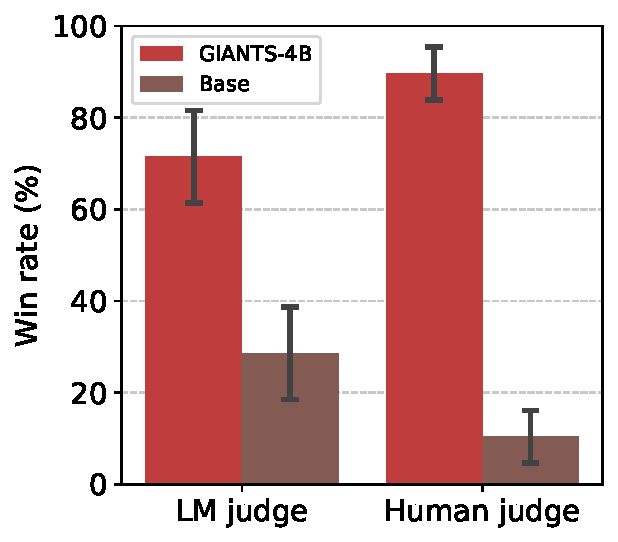
\includegraphics[width=0.9\linewidth]{figs/win_rate_human_eval_similarity.pdf}
    \vspace{-3mm}
    \caption{\footnotesize \textbf{Win rates for \ourmethod{}} \ourmethod{} achieves a higher win rate for similarity than the base model for both the LM and Human judge.} 
    \vspace{-3mm}
    \label{fig:win_rate_human_eval_similarity}
\end{wrapfigure}
\textbf{1) Insights generation is a challenging task even for large proprietary models.} Despite their success across diverse NLP benchmarks, current frontier models exhibit significant limitations in native idea synthesis. For instance, \qwenfourb{} achieves an average similarity score of only $4.75$ (Figure~\ref{fig:all_domain_radar_comparison_gemini-3-pro-preview_vs_Qwen3-14B}). Based on our LLM-based evaluation rubric (Figure~\ref{fig:similarity_judge_prompt}), a score in this range indicates that while generated insights may align topically with the ground truth, they fail to capture the core scientific contribution or technical nuance. Notably, significantly larger proprietary models, such as \gemtwopro{} and \gemthreepro{}, perform similarly to the smaller \qwenfourb{} baseline. This finding suggests that scientific ideation capabilities do not scale linearly with model size alone, reinforcing the necessity for specialized training paradigms like \ourmethod{}.

\begin{wrapfigure}{r}{0.4\textwidth}
    \centering
    \vspace{-2mm}
    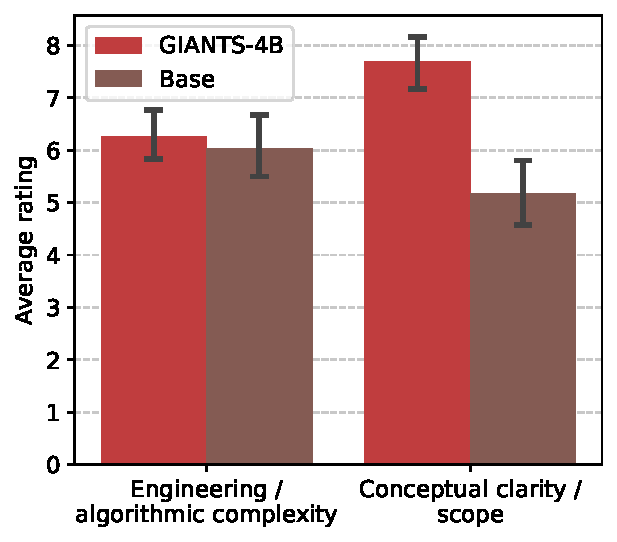
\includegraphics[width=0.9\linewidth]{figs/feasibility_bar_plot.pdf}
    \vspace{-3mm}
    \caption{\footnotesize \textbf{Feasibility Human Eval} Humans gauge the feasibility of a generated insight in 2 axes: (1) engineering/algorithmic complexity \& (2) conceptual clarity/scope, finding \ourmethod{} generates insights with similar algorithmic complexity and better clarity.} 
    \vspace{-3mm}
    \label{fig:feasibility_bar_plot}
\end{wrapfigure}
\textbf{2) Directly optimizing similarity scores significantly improves insight generation}
Our primary finding is that \ourmethod{} achieves the highest performance among all tested methods. By directly optimizing for similarity scores via reinforcement learning (RL), \ourmethod{} yields a relative improvement of 28\% on the full test set (Figure~\ref{fig:all_domain_radar_comparison_gemini-3-pro-preview_vs_Qwen3-14B}) and 34\% on the subset containing only unseen parent papers (Figure~\ref{fig:all_domain_radar_comparison_gemini-3-pro-preview_vs_Qwen3-14B_unseen_parents}) over \gemthreepro{}. In contrast, standard supervised fine-tuning (SFT) on ground-truth insights actually degrades performance, while the SFT-think variant only achieves parity with the base model. These results suggest that standard imitation learning is largely ineffective for this synthesis task; however, our RL framework successfully aligns the model's capabilities with high-quality human insights. This performance trend remains robust as we increase the number of samples to optimize the similarity score via inference-time scaling, as illustrated in Figure~\ref{fig:best_at_k}.

To further validate these gains, we employed the judge framework from \citet{tong2026ai} as an independent third-party evaluation of paper quality. In this setup, the judge model is fine-tuned to predict which of two papers is more likely to receive higher citations. We found that optimizing our similarity-based metric allows \ourmethod{} to achieve a 62\% win rate over the base model across $n=500$ insights across CS disciplines (Figure~\ref{fig:winrate_taste}). This evaluation accounts for potential biases, as in our similarity scoring, by ensuring order invariance and by filtering out inconsistent judgments.

\begin{figure}[t]
    \centering
    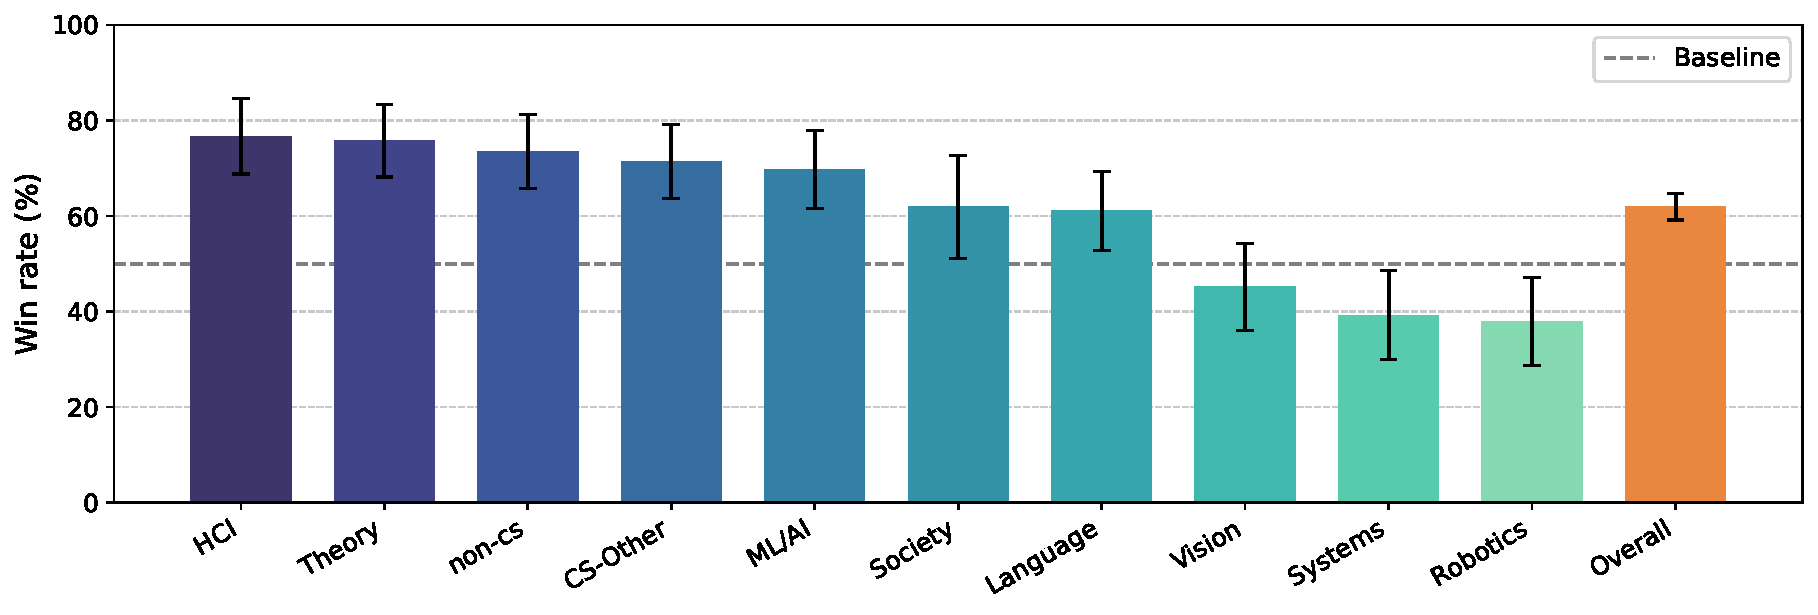
\includegraphics[width=0.9\linewidth]{figs/win_rate_taste_by_domain.pdf}
    \vspace{-3mm}
    \caption{\footnotesize \textbf{\ourmethod{} achieves a 62\% overall win rate against the Base model using SciJudge-30B.} We evaluate \ourmethod{} utilizing the judge framework from \citet{tong2026ai}, originally optimized for citation count prediction. While performance varies by domain, reaching up to a 76\% win rate in HCI but dropping to 37\% in robotics, \ourmethod{} maintains a robust overall win rate of 62\%.}
    \label{fig:winrate_taste}
    \vspace{-3mm}
\end{figure}
We supplemented this automated evaluation with two independent preliminary human studies to assess the real-world impact of our method. First, we measured the win rate of \ourmethod{} against the base model specifically regarding alignment with the downstream paper's actual insights (Figure~\ref{fig:win_rate_human_eval_similarity}). In this head-to-head comparison, \ourmethod{} achieved a $71.4\%$ win rate according to an LM judge and a $89.7\%$ win rate according to human evaluators. Finally, we assessed the feasibility of the generated insights across two axes: algorithmic complexity and conceptual clarity. Our analysis indicates that while \ourmethod{} produces insights of similar algorithmic complexity to the base model, it significantly improves conceptual clarity, making the generated ideas more interpretable and actionable. Further details regarding the human study methodology are provided in Appendix~\ref{app:human_eval}.

\begin{wrapfigure}{r}{0.4\textwidth}
    \centering
    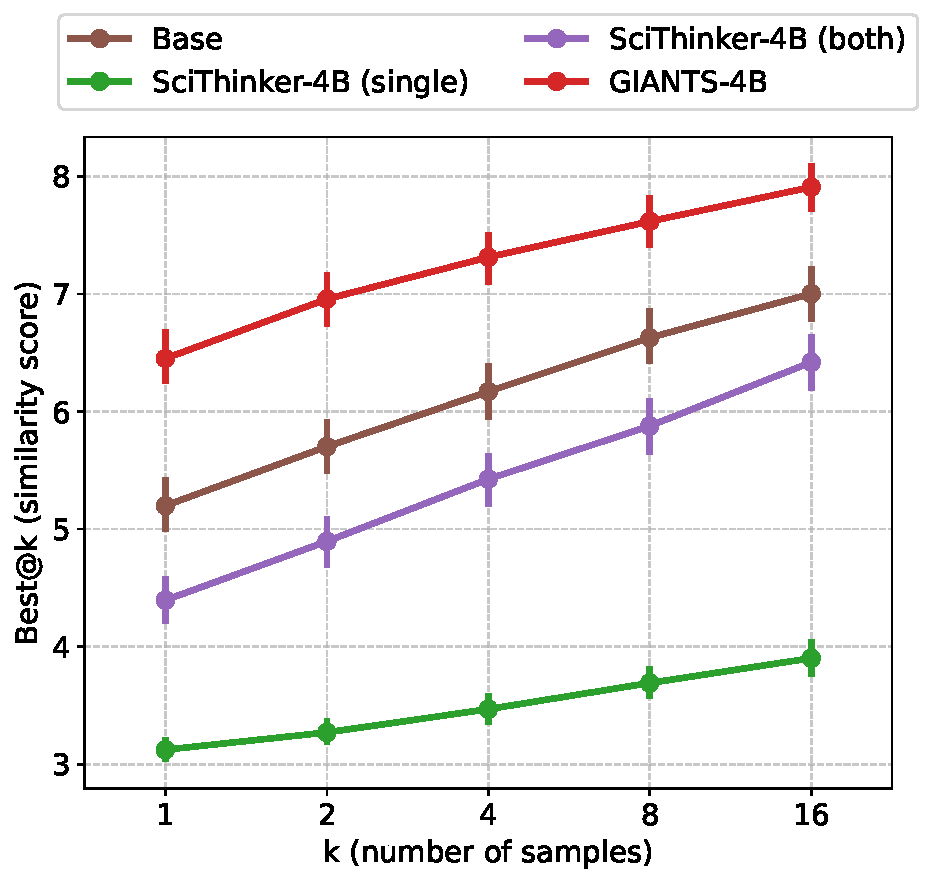
\includegraphics[width=\linewidth]{figs/best_at_k.pdf}
    \vspace{-3mm}
    \caption{\footnotesize \textbf{Test Time Inference of \ourmethod{}}. \ourmethod{} consistently outperforms the base model and other insight proposer methods such as SciThinker-4B~\citep{tong2026ai}, which is optimized for citation count (provided a single or both parent papers).}
    \vspace{-5mm}
    \label{fig:best_at_k}
\end{wrapfigure}
\textbf{3) \ourmethod{} zero-shot generalizes to new domains and distribution of parent papers}. 
Crucially, the synthesis capabilities acquired by \ourmethod{} are not restricted to its training data. Although trained exclusively on papers from the Language domain (CS.CL), we observed consistent performance gains across all evaluated disciplines as seen in Figure~\ref{fig:all_domain_radar_comparison_gemini-3-pro-preview_vs_Qwen3-14B}, including Physics, Quantitative Biology, and Economics. This suggests that the model learns a generalizable mechanism for combining disparate ideas rather than memorizing domain-specific heuristics. Furthermore, Figure~\ref{fig:all_domain_radar_comparison_gemini-3-pro-preview_vs_Qwen3-14B} and \ref{fig:all_domain_radar_comparison_gemini-3-pro-preview_vs_Qwen3-14B_unseen_parents} show the generalization on fully held out papers that appear temporally after the distribution of papers in the training set. 

% Has a lot of whitespace
% \begin{figure}[t]
%     \centering
%     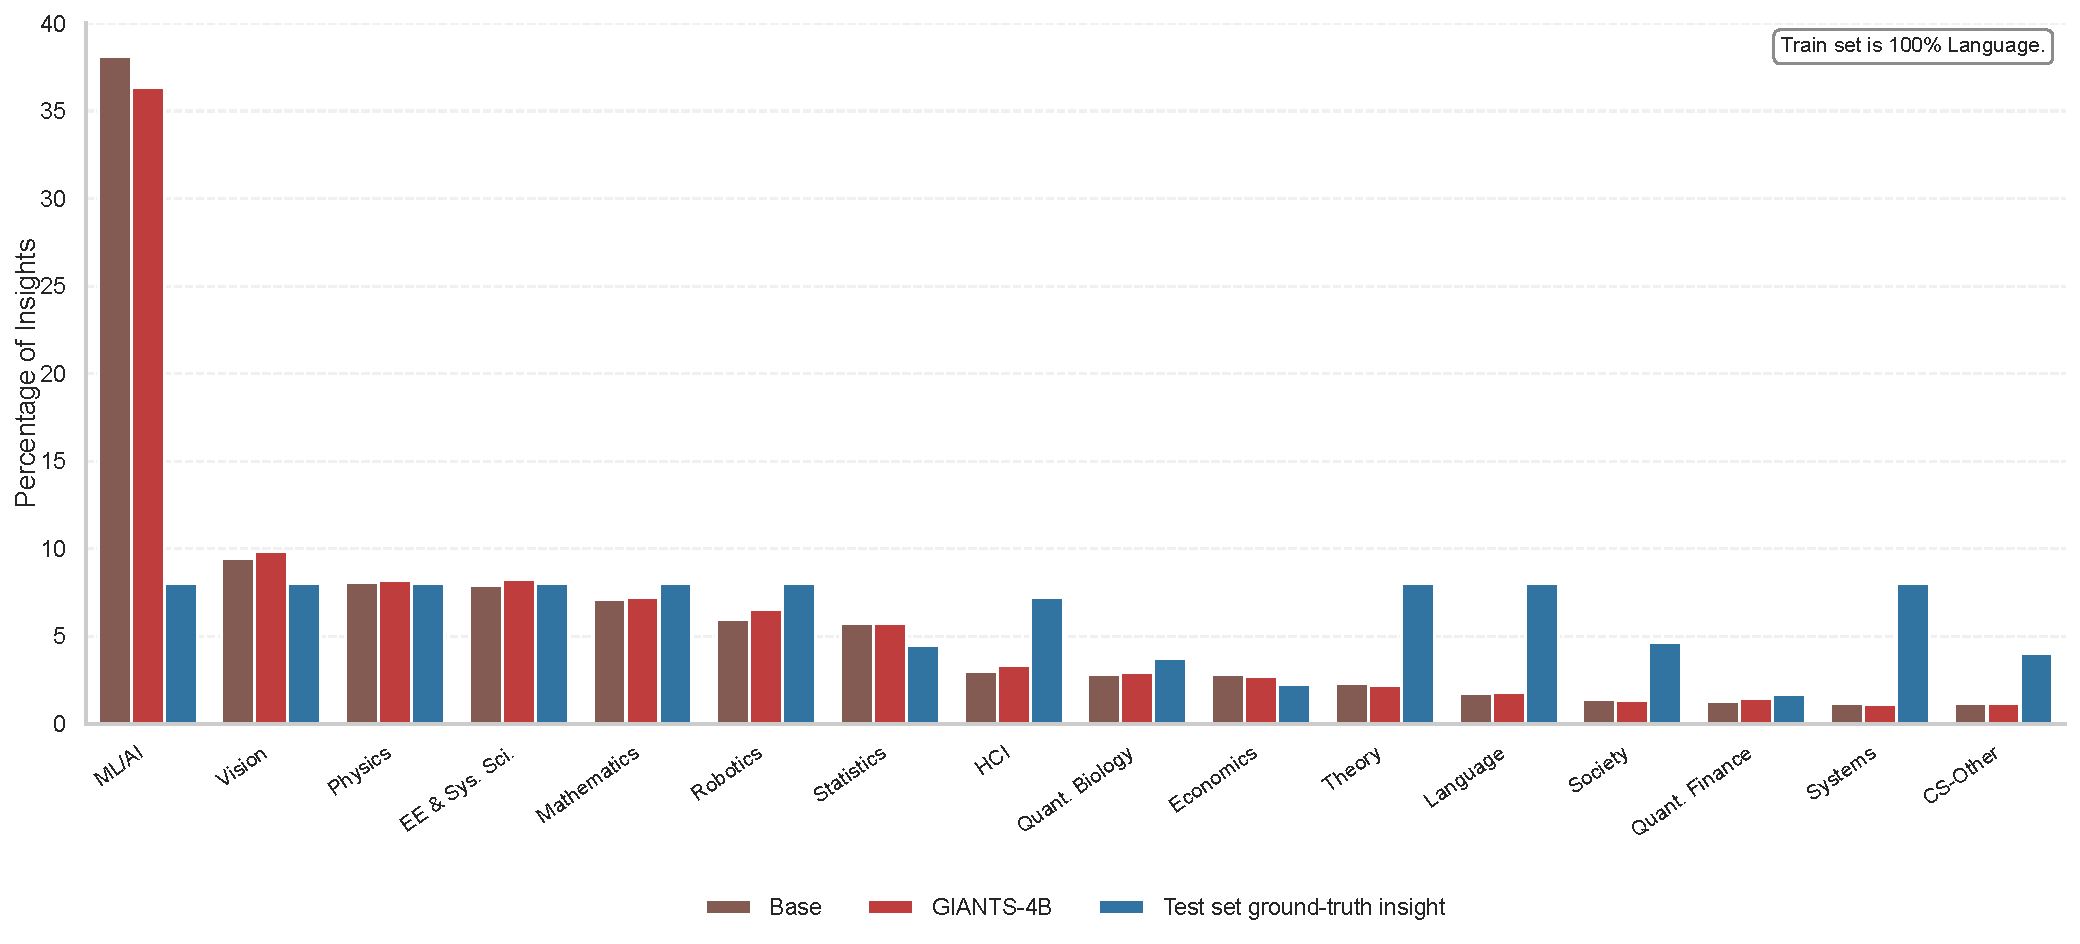
\includegraphics[width=0.9\linewidth]{figs/arxiv_distribution_plot_colorfix.pdf}
%     \vspace{-3mm}
%     \caption{\footnotesize \textbf{The diversity of insights generated by the base and RL models characterized by Gemini 3.1 Flash Lite.} RL fine-tuning for \ourmethod{} keeps a similar distribution of papers to the base model, despite being optimized solely on one domain (cs.CL).}
%     \vspace{-3mm}
%     \label{fig:arxiv_dist}
% \end{figure}

\textbf{Evaluation reliability check}. 
To ensure our findings are robust and that similarity scores are not biased toward the specific judge model that was used during training, we conducted a cross-model validation using an independent judge, \qwenfourteenb{} (Figure~\ref{fig:all_domain_radar_comparison_gemini-3-pro-preview_vs_Qwen3-14B}, right). This secondary evaluation corroborated our primary findings, ranking \ourmethod{} as the top-performing model across all metrics, albeit with a slightly more compressed performance margin. We also report results under three additional judge models in Appendix~\ref{appendix:ablations_with_diverse_lm_judges}, with consistent findings across model sizes.


% \begin{table}[t]
% \begin{center}
% \begin{tabular}{ll}
% \toprule
% \multicolumn{1}{c}{\bf Model}  &\multicolumn{1}{c}{\bf Similarity score on test} \\
% \midrule
% Base (\qwenfourb)         &$6.6$ \\
% RL (\qwenfourb)             &$7.64$ \\
% SFT (\qwenfourb)
% &$6.456$ \\

% SFT-think (\qwenfourb)
% &$6.674$ \\
% \gemtwopro            &$6.903$ \\   
% \gemthreepro             &$6.866$ \\ 
% \bottomrule
% \end{tabular}
% \end{center}\caption{RL outperforms the base model and other frontier models}\label{sample-table}
% \end{table}



% \begin{table}[t]
% \begin{center}
% \begin{tabular}{lcc}
% \toprule
% \multicolumn{1}{c}{\bf Model} 
% & \multicolumn{1}{c}{\bf Similarity score on test (judged by \qwenfourteenb{})} 
% & \multicolumn{1}{c}{\bf Similarity on test-unseen-parents ($N=341$)} \\
% \midrule
% Base (\qwenfourb)        & $7.174$   & $0$ \\
% % SFT (\qwenfourb)         & $6.456$ & $6.468$ \\
% % SFT-think (\qwenfourb)   & $6.674$ & $6.744$ \\
% % \gemtwopro{}               & $6.903$ & $7.038$ \\   
% \gemthreepro{}             & $7.229$ & $0$ \\ 
% RL (\qwenfourb)          & $\textbf{7.594}$  & $0$ \\
% \midrule
% \textit{Relative gain vs.\ Base (RL)} 
% & $\mathbf{+5.9\%}$ 
% & $\mathbf{0}$ \\
% \bottomrule
% \end{tabular}
% \end{center}
% \caption{RL outperforms the base model and other frontier models}
% \label{sample-table}
% \end{table}

% \begin{table}[t]
% \begin{center}
% \begin{tabular}{lcc}
% \toprule
% \multicolumn{1}{c}{\bf Model} 
% & \multicolumn{1}{c}{\bf Similarity score on test (judged by \gemtwopro{})} 
% & \multicolumn{1}{c}{\bf Similarity on test-unseen-parents ($N=341$)} \\
% \midrule
% Base (\qwenfourb)        & $6.526$   & $0$ \\
% % SFT (\qwenfourb)         & $6.456$ & $6.468$ \\
% % SFT-think (\qwenfourb)   & $6.674$ & $6.744$ \\
% % \gemtwopro{}               & $6.903$ & $7.038$ \\   
% \gemthreepro{}             & $6.948$ & $0$ \\ 
% RL (\qwenfourb)          & $\textbf{8.061}$  & $0$ \\
% \midrule
% \textit{Relative gain vs.\ Base (RL)} 
% & $\mathbf{+5.9\%}$ 
% & $\mathbf{0}$ \\
% \bottomrule
% \end{tabular}
% \end{center}
% \caption{RL outperforms the base model and other frontier models}
% \label{sample-table}
% \end{table}

% \begin{figure}[t]
% \begin{center}
% %\framebox[4.0in]{$\;$}
% \fbox{\rule[-.5cm]{0cm}{4cm} \rule[-.5cm]{4cm}{0cm}}
% \end{center}
% \caption{Sample figure caption.}
% \end{figure}
\begin{figure}[t]
    \centering
    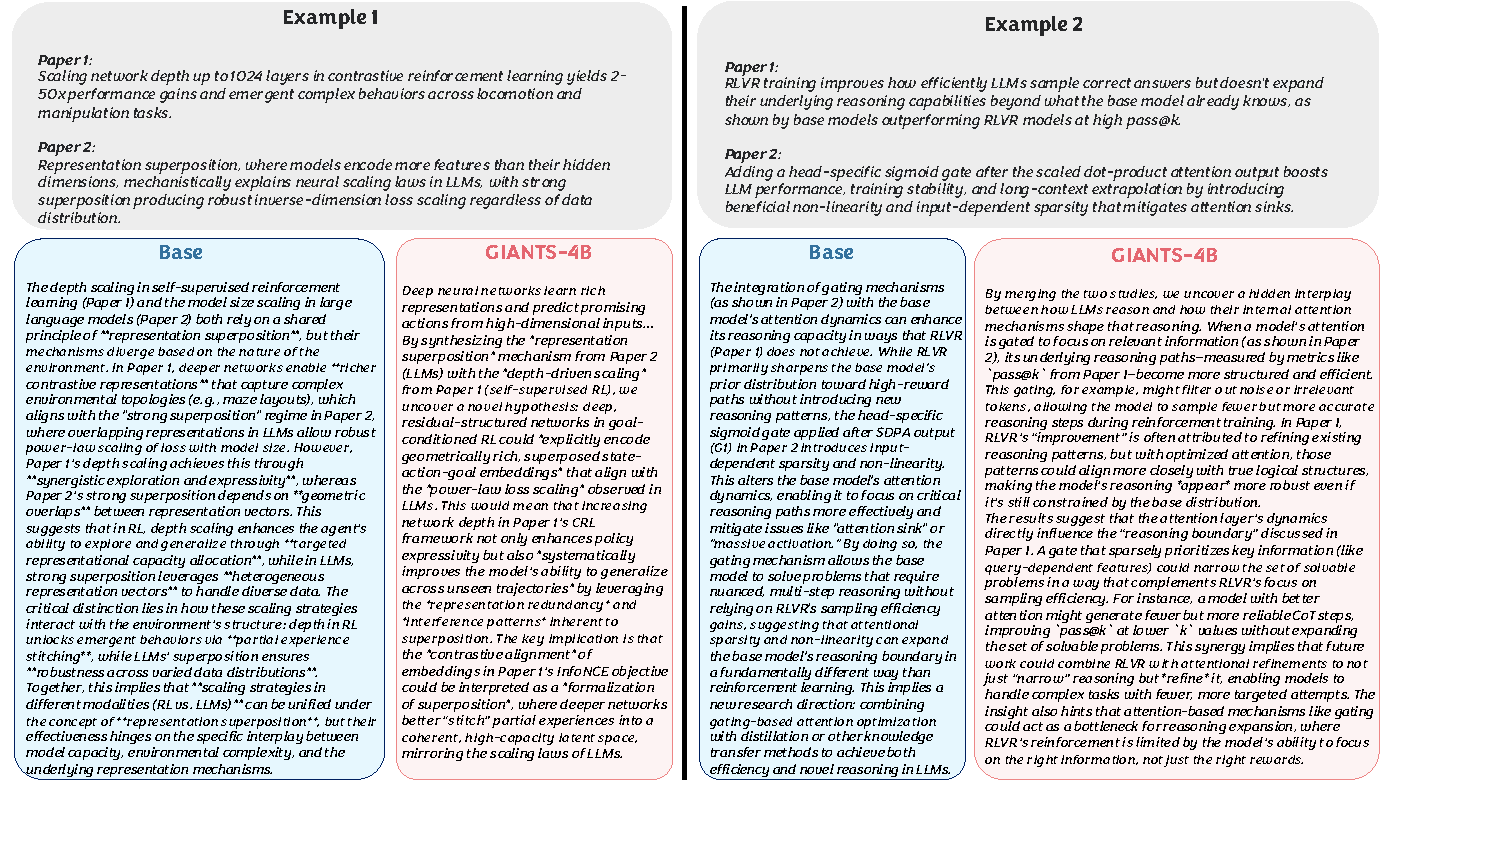
\includegraphics[width=\linewidth]{figs/qualitative.pdf}
    % 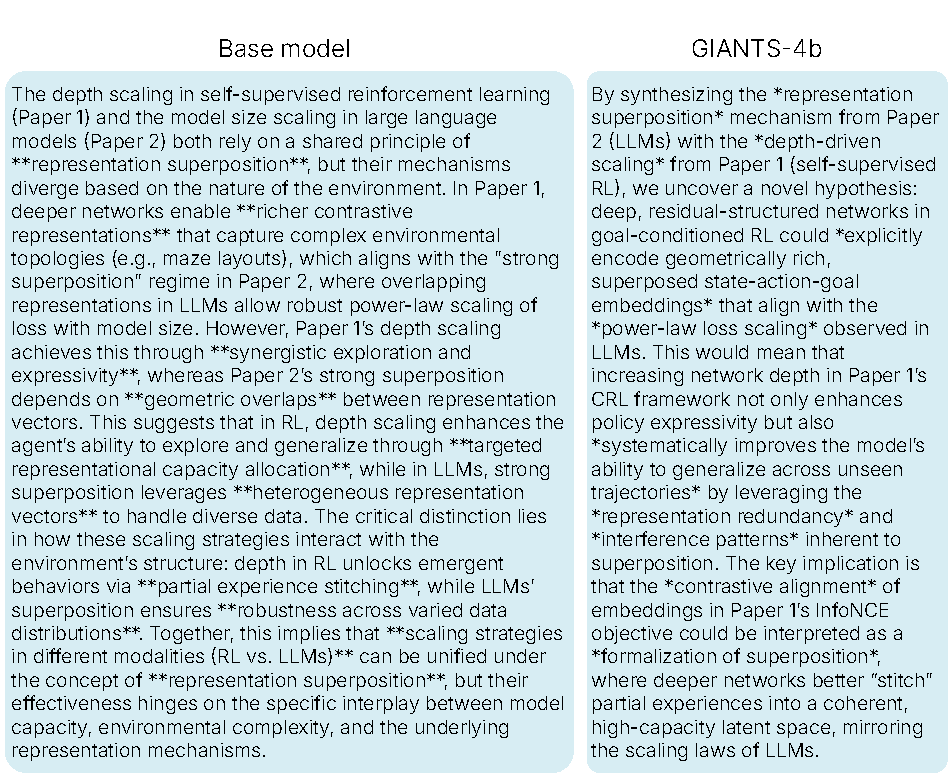
\includegraphics[width=0.43\linewidth]{figs/qualitative_1.pdf}
    % \hspace{3mm} \vrule \hspace{3mm}
    % 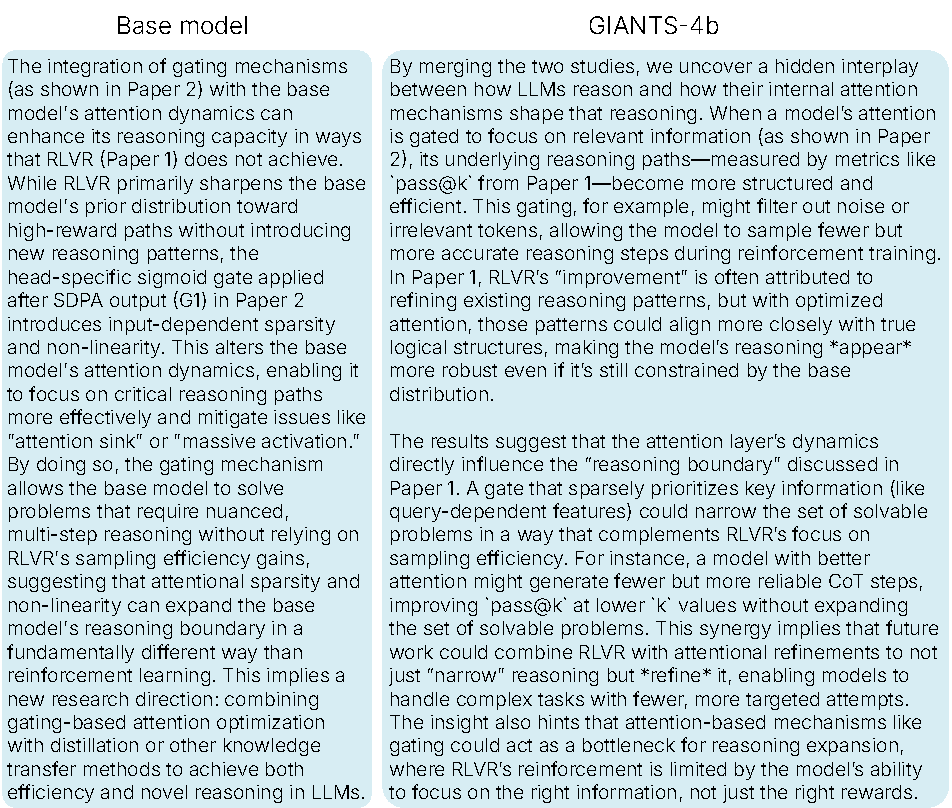
\includegraphics[width=0.4\linewidth]{figs/qualitative_2.pdf}
    \vspace{-3mm}
    \caption{\footnotesize \textbf{Qualitative comparison of insights derived from NeurIPS 2025 award-winning papers.} (Left) \ourmethod{} identifies a more concrete cross-paper mechanism than the base model (\qwenfourb{}). (Right) \ourmethod{} produces a grounded, meaningful contribution, avoiding the overly ambitious and infeasible propositions generated by the base model.}
    \label{fig:qualitative}
    \vspace{-3mm}
\end{figure}
\textbf{Qualitative Comparison of Models}
We present qualitative examples to demonstrate that our generated insights meaningfully integrate concepts from prior literature. To study this, we use NeurIPS 2025 award-winning papers as representative high-quality source material and compare the insights produced by \ourmethod{} against those generated by \qwenfourb{}.

First, Figure~\ref{fig:qualitative} (left) highlights an insight derived from two prior works \citep{wang20251000, liu2025superposition}. While the base model merely summarizes the parent papers without synthesizing a novel perspective, \ourmethod{} proposes a concrete mechanistic connection between the two studies that goes beyond the parent papers. Next, Figure~\ref{fig:qualitative}  (right) examines an insight based on two different papers \citep{yue2025does, qiu2025gated}. Here, the base model generates an overly ambitious claim, suggesting that gating mechanisms expand reasoning boundaries in ways that RLVR cannot, which is unsupported by the source texts. In contrast, \ourmethod{} remains grounded in the actual findings while still identifying a non-trivial connection: that attention gating may dictate how effectively reinforcement learning concentrates probability mass across useful reasoning trajectories. This comparison underscores a critical distinction between boldness and genuine insightfulness. Whereas the base model's novelty relies on unsupported extrapolation, \ourmethod{} maintains a narrower scope to identify a highly plausible interaction between the foundational works.

Overall, these two examples showcase the qualitative differences between the base model and \ourmethod{}, underscoring the properties of diversity and feasibility that are present in the insights that are generated.

\begin{AIbox}{Takeaways of Experimental Evaluation}
\ourmethod{} significantly outperforms both frontier models and supervised fine-tuning at generating feasible, high-quality scientific insights. Furthermore, despite training exclusively on a single domain, the model successfully zero-shot generalizes its synthesis capabilities across diverse, unseen scientific disciplines and temporally held-out literature.
\end{AIbox}





\section{Related Work}
\paragraph{AI for Research.}
Many works have studied how to use LMs for different components of the scientific research pipeline, including literature search \citep{openai_deep_research, zheng-etal-2025-deepresearcher}, idea generation \citep{si2024can, wang-etal-2024-scimon}, and idea execution \citep{si2025ideation, si2026towards, karpathy2026autoresearch}. A concurrent work trains models to judge research impact from citation signals, then uses the learned judge as a reward model for idea generation \citep{tong2026ai}. In contrast, we focus on the problem of synthesizing insights from two parent papers, using similarity to ground-truth downstream insights as a more direct training signal. A recent line of work studies scientific progress as a forecasting problem. Most closely related concurrent work introduces \textsc{PreScience}, a benchmark that decomposes the research process into collaborator prediction, prior work selection, contribution generation, and impact prediction \citep{ajith2026prescience}. In their contribution generation task, models generate a future paper's title and abstract conditioned on prior work and other historical context, and are evaluated using an LM-based similarity metric. Our work is complementary but more focused: rather than modeling the full scientific workflow, we isolate the idea-synthesis problem and ask whether a model can generate the core insight of a downstream paper from a given pair of parent papers. Thus, while \textsc{PreScience} studies broad scientific forecasting, we study a more controlled and direct test of whether models can synthesize a novel downstream insight from specific prior works.


\paragraph{Literature-based Discovery.}
Literature-Based Discovery (LBD) is a field that involves using computational methods to uncover hidden links between seemingly unrelated bodies of research, aiming to infer novel and interesting knowledge \citep{swanson1986fish, swanson2008literature}. For instance, \cite{swanson1986undiscovered} noticed that papers on fish oil mentioned it reduces blood viscosity, while others linked high blood viscosity to Raynaud’s syndrome. Therefore, \cite{swanson1986undiscovered} hypothesized that fish oil could treat Raynaud’s, a prediction later confirmed by clinical research. However, existing LBD approaches struggle to scale to the massive volume of today’s literature and often rely on domain-specific knowledge sources. Moreover, they typically output only ranked lists of candidate connections rather than clear, hypothesis-like insights that researchers can act on \citep{sebastian2017emerging, ganiz2005recent, bekhuis2006conceptual, smalheiser2012literature}. 

% Scientific discovery often depends on synthesizing information across diverse sources to generate novel hypotheses or insights that are not explicitly stated in any single document \citep{swanson1991complementary}. 
\section{Discussion, Limitations, Future Work}
In this work, we introduced \emph{insight anticipation} as a measurable paradigm for automated scientific discovery. By isolating the insight generation phase, we demonstrated that models can effectively synthesize the core insight of a downstream paper when provided with its foundational parent papers. Our results using \ourmethod{} indicate that the trajectory of scientific intuition is partially predictable, and that optimizing language models via reinforcement learning with similarity-based rewards is a highly effective training strategy for this task. However, this foundational formulation leaves several important limitations and open questions.

One limitation of the work is that we assume that downstream contributions derive from two parent papers due to context constraints, despite research ideas being heavily shaped by broader intellectual contexts. Furthermore, parent identification is imperfect. Citations do not always reflect true conceptual influence, and influential ideas may remain uncited. Finally, by assuming an oracle literature selection criterion, we explicitly decoupled insight generation from parent selection, which may not be feasible for some scientific tasks.

Future research can integrate automated retrieval systems to unify parent selection and synthesis within a single end-to-end framework. Additionally, extending the task to accommodate multi-source lineage and developing evaluation metrics that prioritize conceptual novelty over textual similarity could be interesting. Ultimately, testing these models in active, human-in-the-loop research settings will determine their true potential as catalysts for scientific discovery.



% First, to enable controlled evaluation within \ourbenchmark{}, our abstractions assume that downstream contributions derive from exactly two parent papers. While this pairwise framing successfully isolates the mechanics of targeted synthesis, real-world scientific breakthroughs are rarely so cleanly decomposable. Research ideas are heavily shaped by broader intellectual contexts, encompassing multiple prior works, tacit domain knowledge, and evolving community trends. Constricting the lineage to two parents underestimates the complexity of true ideation and may bias models toward overly simplistic, pairwise reasoning patterns.

% Even within our constrained setup, parent identification is imperfect. Citations do not always reflect true conceptual influence, and influential ideas may remain uncited. Conversely, some citations serve rhetorical or historical purposes rather than indicating substantive intellectual dependence. As a result, the mapping from cited parents to “true” idea sources is noisy. This noise places an upper bound on achievable performance and complicates interpretation of both model errors and evaluation scores.

% We explicitly isolate insight synthesis from parent selection by assuming that relevant parents are given. However, selecting which prior work to build upon is itself a central component of scientific reasoning. 

% Our approach has several limitations:
% \begin{itemize}
%     \item Real papers often draw from many influences, whereas we restrict attention to two parents.
%     \item Not all influential ideas are explicitly cited, introducing noise into parent identification.
%     \item Parent selection is assumed to be given and is not modeled.
% \end{itemize}



% This work provides evidence that scientific insight synthesis is partially predictable and that reinforcement learning is particularly well-suited for modeling this process.

% Future directions include scaling to more parent papers, jointly modeling parent selection and idea synthesis, and studying whether models can anticipate emerging research directions rather than reconstructing known ones.
\vspace{-0.15cm}
\section{Ethics Statement}
\vspace{-0.15cm}
This research involves training the \ourmethod{} model on a dataset of 17,839 publicly available arXiv pre-prints to synthesize scientific insights. While automating scientific ideation offers significant potential for discovery, it raises important ethical considerations regarding the proper attribution of foundational ideas, especially since academic citation graphs can be noisy and may not always reflect true conceptual influence. Additionally, there is an inherent risk of language models generating plausible but unverified scientific claims; our framework mitigates this by using reinforcement learning to directly align model outputs with grounded, human-derived insights. Finally, we acknowledge the environmental and computational costs associated with training models on high-performance GPUs, though utilizing a more efficient 4B parameter architecture helps limit this footprint compared to massive proprietary models.


\vspace{-0.15cm}
\section{Reproducibility Statement}
\vspace{-0.15cm}
To ensure the reproducibility of our results, we provide a comprehensive account of our methodology, code, and data. The source code for our models and experiments is available in the supplementary materials and at the following repository: \url{https://github.com/} and a subsample of our benchmark and model weights can be found in the following huggingface respository: \url{https://huggingface.co/giants2026}. Our implementation is built upon the verl framework (\url{https://verl.readthedocs.io/en/latest/}). All experimental details, including hyperparameter settings, are documented in Appendix~\ref{app:hyperparameters}. The computational experiments were conducted on a machine with NVIDIA A100 GPUs, and the required software dependencies are listed in the requirements.txt file within our code repository. The datasets used in our experiments will be made publicly available. We include samples of the dataset in the Appendix along with specific splits and any preprocessing steps applied to the data.

\section{Acknowledgments}
We thank Shirley Wu, Chenglei Si, Ryan Louie, Rui Li, Aviral Kumar, and Andreas Stuhlmüller and others in the Stanford Coco Labs and Iris Labs for discussions and feedback. This work was supported by the Junglee Corporation Stanford Graduate Fellowship. AS gratefully acknowledges the support of the NSF Graduate Research Fellowship Program. CF was supported by Schmidt Sciences.


\clearpage

\bibliography{main}

\newpage
\appendix
\onecolumn

\section{arXiv Paper Domain Classification}
\label{appendix:domain_mapping}
We use the \href{https://arxiv.org/category_taxonomy}{arXiv category taxonomy}. Since Computer Science has many subfields, we further group the arXiv category labels into broader macro-domains.
\begin{table}[htbp]
\centering
\resizebox{\textwidth}{!}{%
\begin{tabular}{ll}
\toprule
\textbf{Domain} & \textbf{arXiv Labels} \\
\midrule
Language & cs.CL \\
ML/AI & cs.LG, cs.AI, cs.NE, cs.MA \\
Robotics & cs.RO \\
Vision & cs.CV, cs.GR, cs.MM, cs.SD \\
Theory & cs.CC, cs.DS, cs.FL, cs.LO, cs.DM, cs.CG, cs.GT, cs.CR, cs.IT \\
Systems & cs.AR, cs.OS, cs.DC, cs.NI, cs.PF, cs.SY, cs.PL, cs.SE, cs.DB, cs.IR, cs.SI \\
Society & cs.CY \\
HCI & cs.HC \\
CS-Other & cs.ET, cs.GL, cs.OH, cs.DL, cs.NA, cs.MS, cs.CE, cs.SC \\
Economics & econ \\
Electrical Engineering \& Systems Science (EE \& Sys. Sci.) & eess \\
Mathematics & math \\
Physics & astro-ph, cond-mat, gr-qc, hep-ex, hep-lat, hep-ph, hep-th, math-ph, nlin, nucl-ex, nucl-th, physics, quant-ph \\
Quantitative Biology (Quant. Bio.) & q-bio \\
Quantitative Finance (Quant. Fin.) & q-fin \\
Statistics & stat \\
\bottomrule
\end{tabular}%
}
\caption{Mapping from domains to arXiv category labels.}
\label{table:domain_mapping}
\end{table}



\section{Further Quantitative Analysis}

In this section, we provide a more granular, domain-by-domain breakdown of our quantitative results to better understand the performance characteristics of each model across different scientific disciplines. 

Table \ref{table:domain_results} presents the average similarity scores across the entirety of \ourbenchmark{}. The results demonstrate that \ourmethod{} achieves consistent, robust improvements over both the base models and the supervised fine-tuning (SFT) baselines. Notably, this performance gap holds steady across highly diverse fields, ranging from largely theoretical domains like Mathematics and Theory to applied disciplines such as Vision, Robotics, and HCI.

\begin{table}[htbp]
\centering
\resizebox{\textwidth}{!}{%
\begin{tabular}{lcccccc}
\toprule
\textbf{Domain} & \textbf{Base} & \textbf{SFT} & \textbf{SFT-think} & \textbf{\gemtwopro{}} & \textbf{\gemthreepro{}} & \textbf{\ourmethod{}} \\
\midrule
Economics & $4.66_{{\pm0.21}}$ & $4.78_{{\pm0.20}}$ & $4.94_{{\pm0.21}}$ & $4.75_{{\pm0.22}}$ & $4.50_{{\pm0.20}}$ & \textbf{$5.47_{{\pm0.22}}$} \\
Language & $4.50_{{\pm0.10}}$ & $4.75_{{\pm0.10}}$ & $4.84_{{\pm0.11}}$ & $4.45_{{\pm0.11}}$ & $4.14_{{\pm0.10}}$ & \textbf{$5.50_{{\pm0.11}}$} \\
Vision & $4.28_{{\pm0.10}}$ & $4.59_{{\pm0.10}}$ & $4.57_{{\pm0.10}}$ & $4.11_{{\pm0.10}}$ & $4.14_{{\pm0.10}}$ & \textbf{$5.52_{{\pm0.12}}$} \\
Theory & $4.54_{{\pm0.10}}$ & $4.72_{{\pm0.10}}$ & $4.80_{{\pm0.11}}$ & $4.67_{{\pm0.11}}$ & $4.58_{{\pm0.11}}$ & \textbf{$5.63_{{\pm0.11}}$} \\
Mathematics & $4.64_{{\pm0.11}}$ & $4.73_{{\pm0.10}}$ & $4.81_{{\pm0.10}}$ & $4.76_{{\pm0.11}}$ & $4.58_{{\pm0.10}}$ & \textbf{$5.66_{{\pm0.11}}$} \\
Quant. Fin. & $4.82_{{\pm0.25}}$ & $5.15_{{\pm0.23}}$ & $5.31_{{\pm0.25}}$ & $5.04_{{\pm0.26}}$ & $4.45_{{\pm0.24}}$ & \textbf{$5.75_{{\pm0.26}}$} \\
ML/AI & $4.77_{{\pm0.11}}$ & $4.97_{{\pm0.11}}$ & $4.87_{{\pm0.11}}$ & $4.64_{{\pm0.11}}$ & $4.56_{{\pm0.11}}$ & \textbf{$5.76_{{\pm0.12}}$} \\
Systems & $4.62_{{\pm0.11}}$ & $5.07_{{\pm0.11}}$ & $5.13_{{\pm0.11}}$ & $4.57_{{\pm0.11}}$ & $4.41_{{\pm0.11}}$ & \textbf{$6.04_{{\pm0.12}}$} \\
Society & $4.87_{{\pm0.14}}$ & $5.31_{{\pm0.14}}$ & $5.33_{{\pm0.15}}$ & $4.40_{{\pm0.13}}$ & $3.82_{{\pm0.11}}$ & \textbf{$6.05_{{\pm0.15}}$} \\
Physics & $4.82_{{\pm0.11}}$ & $5.27_{{\pm0.11}}$ & $5.30_{{\pm0.11}}$ & $4.95_{{\pm0.11}}$ & $4.65_{{\pm0.11}}$ & \textbf{$6.14_{{\pm0.12}}$} \\
Robotics & $4.74_{{\pm0.11}}$ & $5.06_{{\pm0.11}}$ & $5.11_{{\pm0.11}}$ & $4.55_{{\pm0.11}}$ & $4.43_{{\pm0.11}}$ & \textbf{$6.21_{{\pm0.11}}$} \\
EE \& Sys. & $4.83_{{\pm0.11}}$ & $5.02_{{\pm0.11}}$ & $5.08_{{\pm0.11}}$ & $4.74_{{\pm0.11}}$ & $4.55_{{\pm0.11}}$ & \textbf{$6.22_{{\pm0.12}}$} \\
HCI & $4.95_{{\pm0.12}}$ & $5.12_{{\pm0.11}}$ & $5.02_{{\pm0.11}}$ & $4.52_{{\pm0.11}}$ & $4.01_{{\pm0.10}}$ & \textbf{$6.23_{{\pm0.12}}$} \\
Statistics & $5.45_{{\pm0.16}}$ & $5.38_{{\pm0.15}}$ & $5.51_{{\pm0.15}}$ & $5.50_{{\pm0.16}}$ & $5.68_{{\pm0.17}}$ & \textbf{$6.46_{{\pm0.16}}$} \\
Quant. Bio. & $5.17_{{\pm0.17}}$ & $5.43_{{\pm0.17}}$ & $5.69_{{\pm0.17}}$ & $4.94_{{\pm0.17}}$ & $4.41_{{\pm0.15}}$ & \textbf{$6.65_{{\pm0.17}}$} \\
CS-Other & $5.16_{{\pm0.16}}$ & $5.58_{{\pm0.16}}$ & $5.42_{{\pm0.16}}$ & $4.57_{{\pm0.15}}$ & $4.19_{{\pm0.14}}$ & \textbf{$6.70_{{\pm0.16}}$} \\
\midrule
\textbf{Overall} & $4.75_{{\pm0.03}}$ & $5.01_{{\pm0.03}}$ & $5.05_{{\pm0.03}}$ & $4.65_{{\pm0.03}}$ & $4.43_{{\pm0.03}}$ & \textbf{$5.97_{{\pm0.03}}$} \\
\bottomrule
\end{tabular}%
}
\caption{Average similarity scores (mean $\pm$ standard error) per domain on \ourbenchmark{}. The judge LM is \gemthreepro{}.}
\label{table:domain_results}
\end{table}

To further validate the generalization capabilities of our approach and ensure the model is not merely memorizing training distributions, we separately evaluated performance on a highly constrained subset of the data: \textbf{Test-unseen-parents}. This subset exclusively contains test examples where the parent papers were never encountered during the training phase. 

The results for this holdout set are detailed in Table \ref{table:domain_results_unseen}. Encouragingly, \ourmethod{} maintains its substantial performance gap over the baselines even on unseen literature. This indicates that our model has successfully learned generalized mechanisms for cross-paper insight generation that translate effectively to novel scientific texts.

\begin{table}[htbp]
\centering
\resizebox{\textwidth}{!}{%
\begin{tabular}{lcccccc}
\toprule
\textbf{Domain} & \textbf{Base} & \textbf{SFT} & \textbf{SFT-think} & \textbf{\gemtwopro{}} & \textbf{\gemthreepro{}} & \textbf{\ourmethod{}} \\
\midrule
Economics & $4.63_{{\pm0.22}}$ & $4.73_{{\pm0.21}}$ & $4.93_{{\pm0.21}}$ & $4.76_{{\pm0.23}}$ & $4.55_{{\pm0.21}}$ & \textbf{$5.50_{{\pm0.23}}$} \\
Language & $4.59_{{\pm0.19}}$ & $4.79_{{\pm0.19}}$ & $4.96_{{\pm0.20}}$ & $4.52_{{\pm0.19}}$ & $4.28_{{\pm0.18}}$ & \textbf{$5.62_{{\pm0.20}}$} \\
Vision & $4.45_{{\pm0.14}}$ & $4.57_{{\pm0.15}}$ & $4.64_{{\pm0.14}}$ & $4.14_{{\pm0.14}}$ & $4.33_{{\pm0.15}}$ & \textbf{$5.71_{{\pm0.17}}$} \\
Theory & $4.63_{{\pm0.12}}$ & $4.80_{{\pm0.12}}$ & $4.76_{{\pm0.12}}$ & $4.84_{{\pm0.13}}$ & $4.75_{{\pm0.13}}$ & \textbf{$5.71_{{\pm0.13}}$} \\
Mathematics & $4.63_{{\pm0.11}}$ & $4.72_{{\pm0.10}}$ & $4.80_{{\pm0.10}}$ & $4.74_{{\pm0.11}}$ & $4.57_{{\pm0.10}}$ & \textbf{$5.63_{{\pm0.11}}$} \\
Quant. Fin. & $4.76_{{\pm0.27}}$ & $5.18_{{\pm0.25}}$ & $5.30_{{\pm0.26}}$ & $4.89_{{\pm0.27}}$ & $4.48_{{\pm0.25}}$ & \textbf{$5.77_{{\pm0.27}}$} \\
ML/AI & $4.88_{{\pm0.15}}$ & $5.18_{{\pm0.16}}$ & $4.95_{{\pm0.15}}$ & $4.87_{{\pm0.16}}$ & $4.99_{{\pm0.16}}$ & \textbf{$6.06_{{\pm0.16}}$} \\
Systems & $4.74_{{\pm0.15}}$ & $5.04_{{\pm0.15}}$ & $5.07_{{\pm0.15}}$ & $4.74_{{\pm0.16}}$ & $4.54_{{\pm0.15}}$ & \textbf{$6.15_{{\pm0.16}}$} \\
Society & $4.96_{{\pm0.19}}$ & $5.45_{{\pm0.19}}$ & $5.26_{{\pm0.19}}$ & $4.47_{{\pm0.17}}$ & $3.77_{{\pm0.14}}$ & \textbf{$6.13_{{\pm0.20}}$} \\
Physics & $4.82_{{\pm0.11}}$ & $5.28_{{\pm0.11}}$ & $5.29_{{\pm0.11}}$ & $4.99_{{\pm0.12}}$ & $4.67_{{\pm0.11}}$ & \textbf{$6.16_{{\pm0.12}}$} \\
Robotics & $4.89_{{\pm0.13}}$ & $5.14_{{\pm0.12}}$ & $5.19_{{\pm0.13}}$ & $4.58_{{\pm0.13}}$ & $4.48_{{\pm0.13}}$ & \textbf{$6.34_{{\pm0.13}}$} \\
EE \& Sys. & $4.90_{{\pm0.13}}$ & $5.21_{{\pm0.13}}$ & $5.20_{{\pm0.12}}$ & $4.80_{{\pm0.13}}$ & $4.72_{{\pm0.13}}$ & \textbf{$6.35_{{\pm0.14}}$} \\
HCI & $5.19_{{\pm0.15}}$ & $5.23_{{\pm0.14}}$ & $5.15_{{\pm0.14}}$ & $4.74_{{\pm0.14}}$ & $4.17_{{\pm0.12}}$ & \textbf{$6.41_{{\pm0.15}}$} \\
Statistics & $5.47_{{\pm0.17}}$ & $5.43_{{\pm0.15}}$ & $5.53_{{\pm0.16}}$ & $5.49_{{\pm0.17}}$ & $5.67_{{\pm0.18}}$ & \textbf{$6.51_{{\pm0.16}}$} \\
Quant. Bio. & $5.27_{{\pm0.18}}$ & $5.56_{{\pm0.18}}$ & $5.77_{{\pm0.18}}$ & $5.05_{{\pm0.18}}$ & $4.35_{{\pm0.16}}$ & \textbf{$6.77_{{\pm0.18}}$} \\
CS-Other & $5.38_{{\pm0.19}}$ & $5.65_{{\pm0.18}}$ & $5.50_{{\pm0.18}}$ & $4.66_{{\pm0.17}}$ & $4.20_{{\pm0.16}}$ & \textbf{$6.85_{{\pm0.18}}$} \\
\midrule
\textbf{Overall} & $4.87_{{\pm0.04}}$ & $5.10_{{\pm0.04}}$ & $5.11_{{\pm0.04}}$ & $4.78_{{\pm0.04}}$ & $4.57_{{\pm0.04}}$ & \textbf{$6.11_{{\pm0.04}}$} \\
\bottomrule
\end{tabular}%
}
\caption{Average similarity scores (mean $\pm$ standard error) per domain on  \textbf{Test-unseen-parents}, which indicates the subset of \ourbenchmark{} test set with only unseen parent papers. The judge LLM is \gemthreepro{}.}
\label{table:domain_results_unseen}
\end{table}

\section{Prompts}

This section details the exact prompt templates utilized throughout our pipeline for both generation and evaluation tasks. 

\subsection{Insight Generation Prompt}
\label{appendix:insight_gen_prompt}

Below, the prompt utilized for the insight generation task is listed. The model is provided with the textual summaries of two distinct parent papers, which are highlighted in red in the accompanying figure. The prompt systematically instructs the model to analyze these summaries, synthesize their core methodologies or findings, and autonomously generate a novel scientific insight or proposed research direction that logically bridges and builds upon both foundational works.

\begin{figure}[tb]
    \centering
    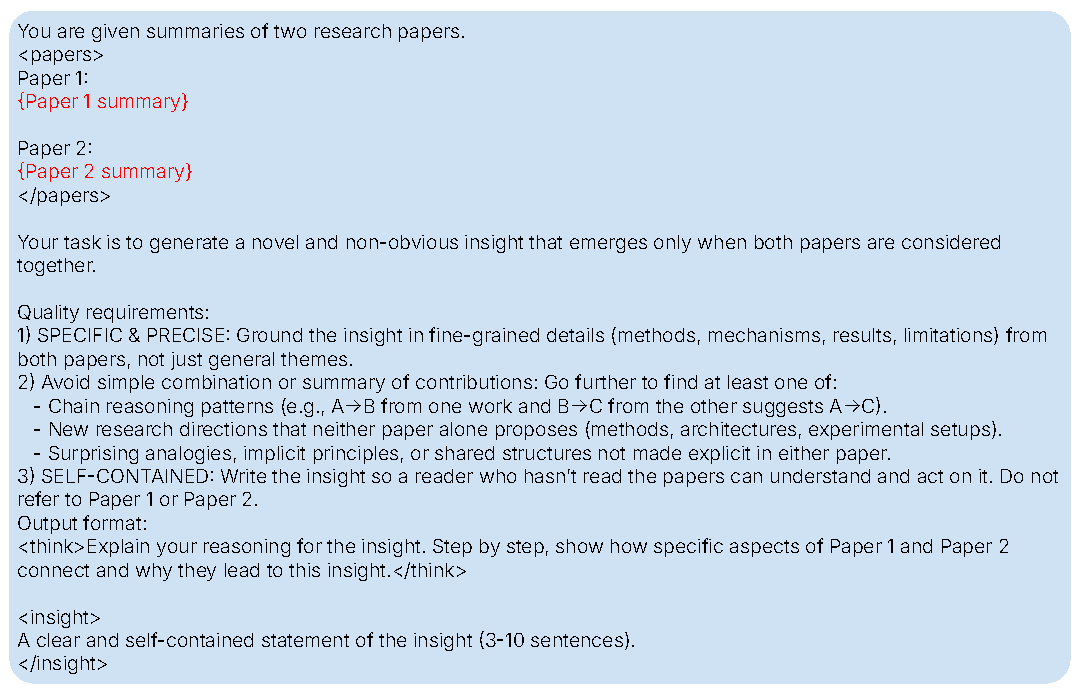
\includegraphics[width=0.95\linewidth]{figs/insight_generation_prompt.pdf}
    % \vspace{-3mm}
    \caption{Prompt for insight generation. The summaries of two parent papers are in \textcolor{red}{red}.}
    \label{fig:insight_generation_prompt}
\end{figure}

\subsection{Ancestor Identification Prompt}
\label{appendix:ancestor_id_prompt}

Here, we present the prompt designed for the ancestor identification task. The primary objective of this prompt is to instruct the model to determine the most influential parent papers for a given downstream target paper. By providing the model with the abstract or conceptual context of the downstream paper, the prompt asks the model to trace the scientific lineage backward and reliably identify which prior works from a candidate pool served as its direct conceptual ancestors.

\begin{figure}[tb]
    \centering
    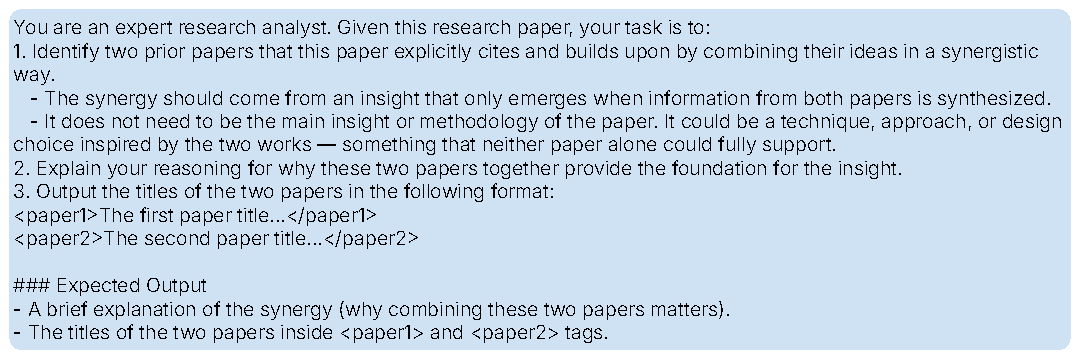
\includegraphics[width=\linewidth]{figs/upstream_citation_prompt.pdf}
    \vspace{-3mm}
    \caption{Prompt for identifying two parent papers whose ideas are synergistically combined to produce the given paper's key insight, which is extracted as the ground-truth target $y^*$.}
    \label{fig:upstream_citation_prompt}
\end{figure}

\subsection{Similarity Judge Prompt}
\label{appendix:similarity_judge_prompt}

Below, we outline the prompt used for automated evaluation and reward scoring via an LLM-as-a-judge framework. To quantitatively assess the quality and relevance of our generated insights, this prompt provides the evaluator model with both the human-verified ground-truth insight and the corresponding model-generated insight. The model is then instructed to critically compare the two texts and output a similarity assessment, evaluating them on semantic alignment, scientific coherence, and the degree of conceptual overlap.

\begin{figure}[t]
    \centering
    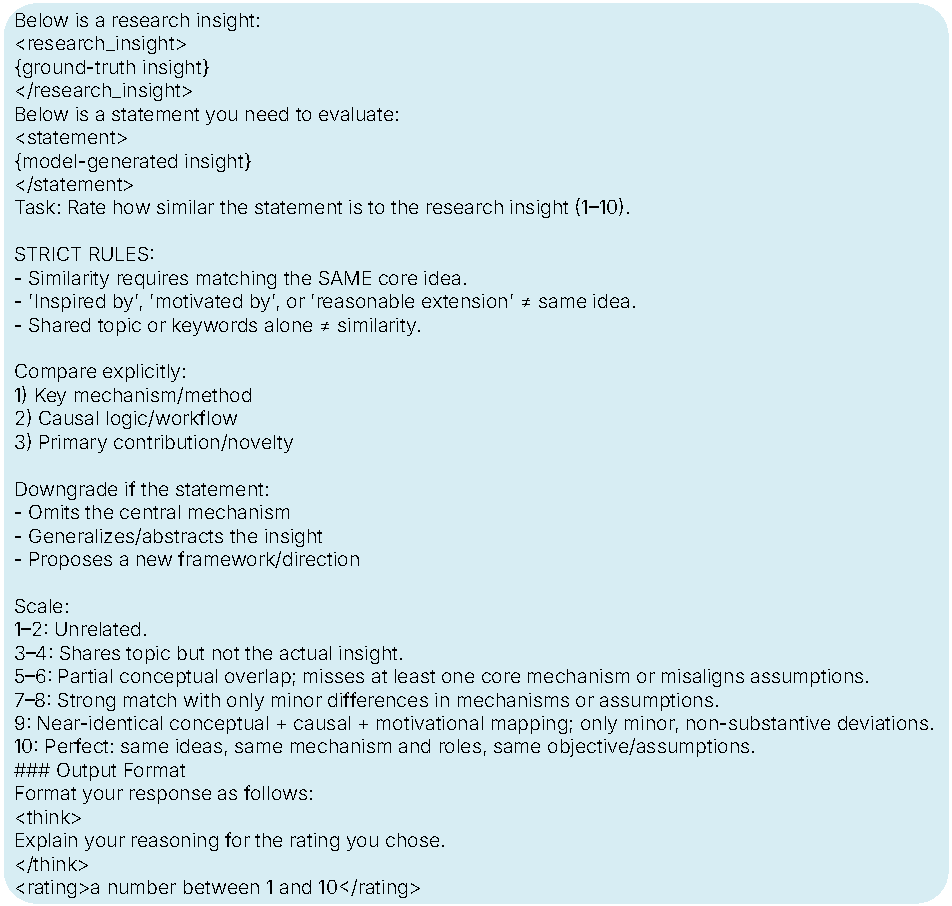
\includegraphics[width=0.6\linewidth]{figs/similarity_judge_prompt.pdf}
    % \vspace{-3mm}
    \caption{Prompt for assessing the similarity between the ground-truth insight and model-generated insight.}
    \label{fig:similarity_judge_prompt}
\end{figure}

\subsection{Rewriting Insight Prompt}
\label{appendix:rewriting_insight_prompt}

To ensure the generated insights could be evaluated consistently, we employed a rewriting step to standardize their format. Figure \ref{fig:rewrite_insight_prompt} displays the prompt used to instruct the model to rewrite the raw insight into a clear, standalone statement without losing its original semantic meaning.

\begin{figure}[H]
    \centering
    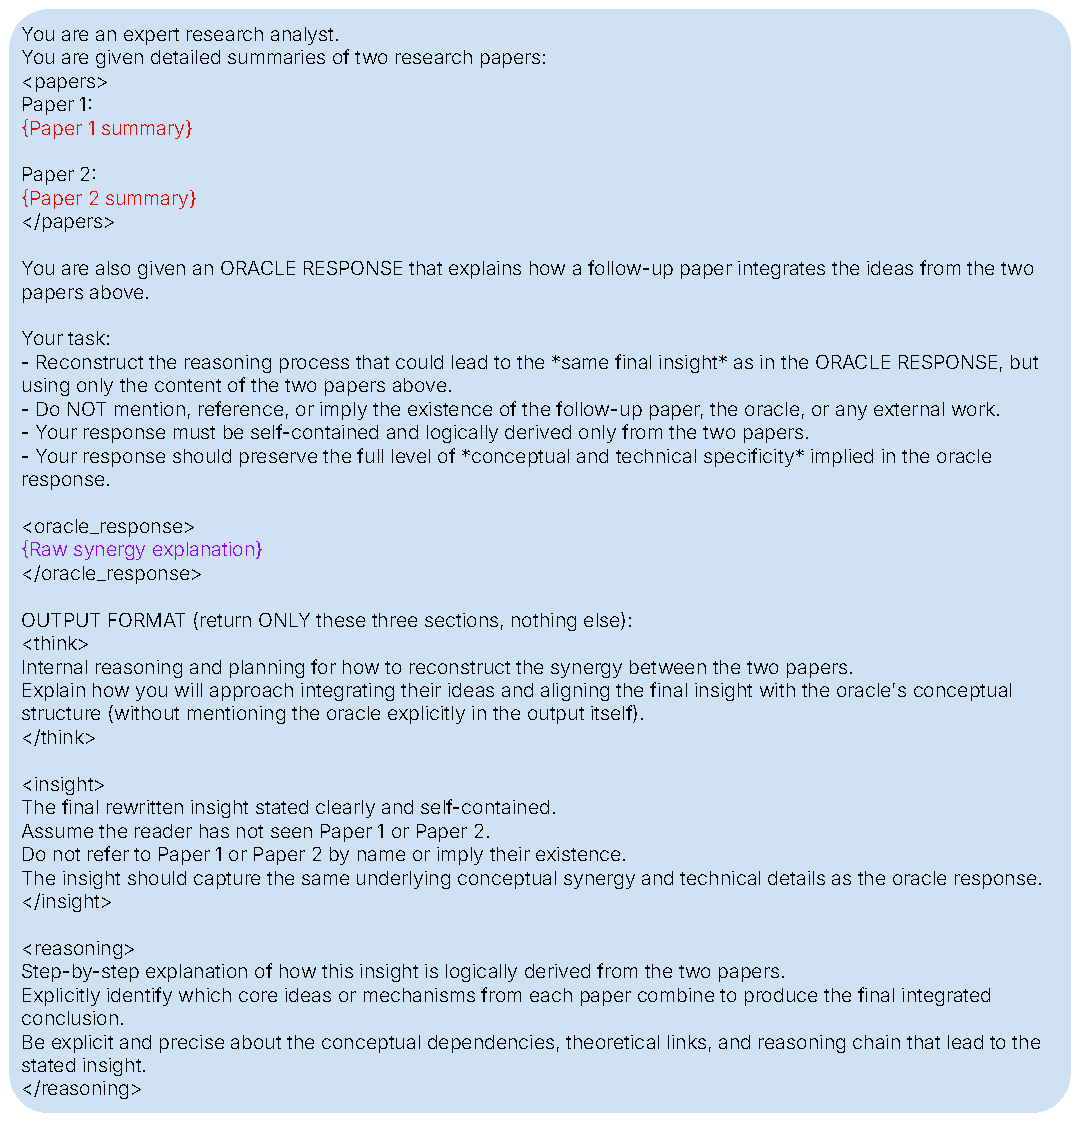
\includegraphics[width=0.6\linewidth]{figs/rewrite_insight_prompt.pdf}
    % \vspace{-3mm}
    \caption{Prompt for rewriting the insight as a standalone statement.}
    \label{fig:rewrite_insight_prompt}
\end{figure}

% \subsection{Similarity Judge Prompt}
% \label{appendix:similarity_judge_prompt}
% \begin{figure}[H]
%     \centering
%     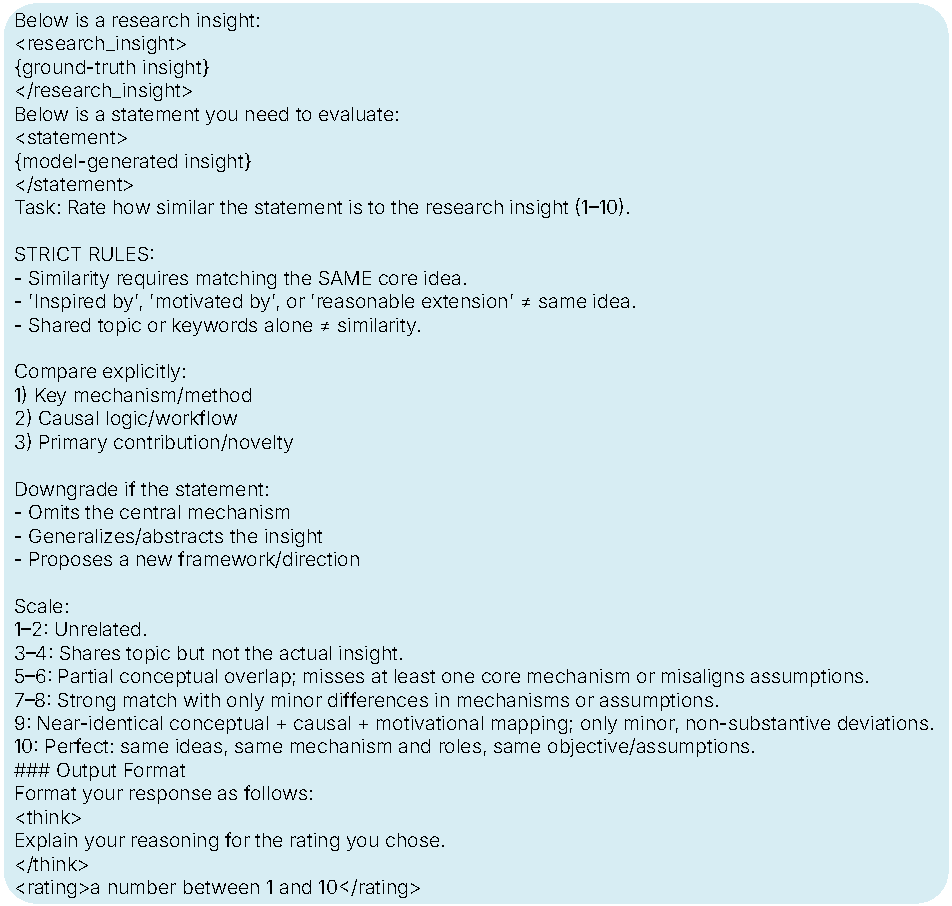
\includegraphics[width=\linewidth]{figs/similarity_judge_prompt.pdf}
%     % \vspace{-3mm}
%     \caption{Prompt for assessing the similarity between the ground-truth insight and model-generated insight.}
%     \label{fig:similarity_judge_prompt}
% \end{figure}

\subsection{Hyperparameters for \ourmethod{} and Baselines}
\label{app:hyperparameters}

We detail the optimization and training configurations used for evaluating \ourmethod{} against the baselines below. The hyperparameter choices were guided by standard practices for aligning large language models, with slight adjustments made to accommodate our specific sequence lengths and batch sizes.

\paragraph{RL Hyperparameters.} 
Table \ref{tab:rl_hyperparameters} outlines the configuration used during the reinforcement learning phase, specifically utilizing the GRPO algorithm. We applied a conservative KL penalty to prevent the model from drifting too far from the reference policy.

\begin{table*}[h]
\centering
\small
\setlength{\tabcolsep}{10pt}
\renewcommand{\arraystretch}{1.15}
\begin{tabularx}{\linewidth}{>{\raggedright\arraybackslash}X >{\centering\arraybackslash}p{0.34\linewidth}}
\toprule
\textbf{Hyperparameter} & \textbf{Value} \\
\midrule
Algorithm                           & GRPO~\citep{shao2024deepseekmath} \\
Training steps                      & 400 \\
Train batch size                    & 64 \\
Group size                          & 8 \\
Max prompt length                   & 3000 \\
Max response length                 & 1296 \\
Learning rate                       & $1\times10^{-6}$ \\
Entropy coefficient                 & 0.001 \\
KL loss coefficient                 & 0.001 \\
KL loss type                        & \texttt{low\_var\_kl} \\
Sampling temperature (train / val)  & 0.6 / 0.6 \\
Samples per prompt (train / val)    & 16 / 8 \\
Max batched tokens                  & 32768 \\
Uneven Clipping (low / high)        & 0.2 / 0.5 \\
\bottomrule
\end{tabularx}
\caption{Key reinforcement learning hyperparameters used in our experiments.}
\label{tab:rl_hyperparameters}
\end{table*}

\paragraph{Supervised Learning Hyperparameters.}
Table \ref{tab:sft_hyperparameters} details the setup for our supervised fine-tuning (SFT) baselines. Where multiple values were explored during our grid search, the final selected optimal configuration is marked in bold.

\begin{table*}[h]
\centering
\small
\setlength{\tabcolsep}{10pt}
\renewcommand{\arraystretch}{1.15}
\begin{tabularx}{\linewidth}{>{\raggedright\arraybackslash}X >{\centering\arraybackslash}p{0.34\linewidth}}
\toprule
\textbf{Hyperparameter} & \textbf{Value} \\
\midrule
Algorithm                           & SFT~\cite{} \\
Epochs                              & 10 \\
Train batch size                    & 64 \\
Max length (input + output)         & 16384 \\
Learning rate                       & $5\times10^{-5}$, $1\times10^{-5}$, \textbf{$5\times10^{-6}$}, $1\times10^{-6}$ \\
Weight decay                        & \textbf{$1\times10^{-2}$}, $1\times10^{-4}$ \\
Sampling temperature (train / val)  & 0.6 / 0.6 \\
Learning rate schedule              & Cosine annealing \\
Learning rate warmup ratio          & 0.01 \\
Gradient checkpointing              & True \\
Gradient accumulation steps         & 16 \\
\bottomrule
\end{tabularx}
\caption{Key supervised fine-tuning hyperparameters used in our experiments. Bold indicates the selected configuration when multiple values were explored.}
\label{tab:sft_hyperparameters}
\end{table*}

\section{Ablations with Diverse LM Judges}
\label{appendix:ablations_with_diverse_lm_judges}

\begin{figure}[H]
    \centering
    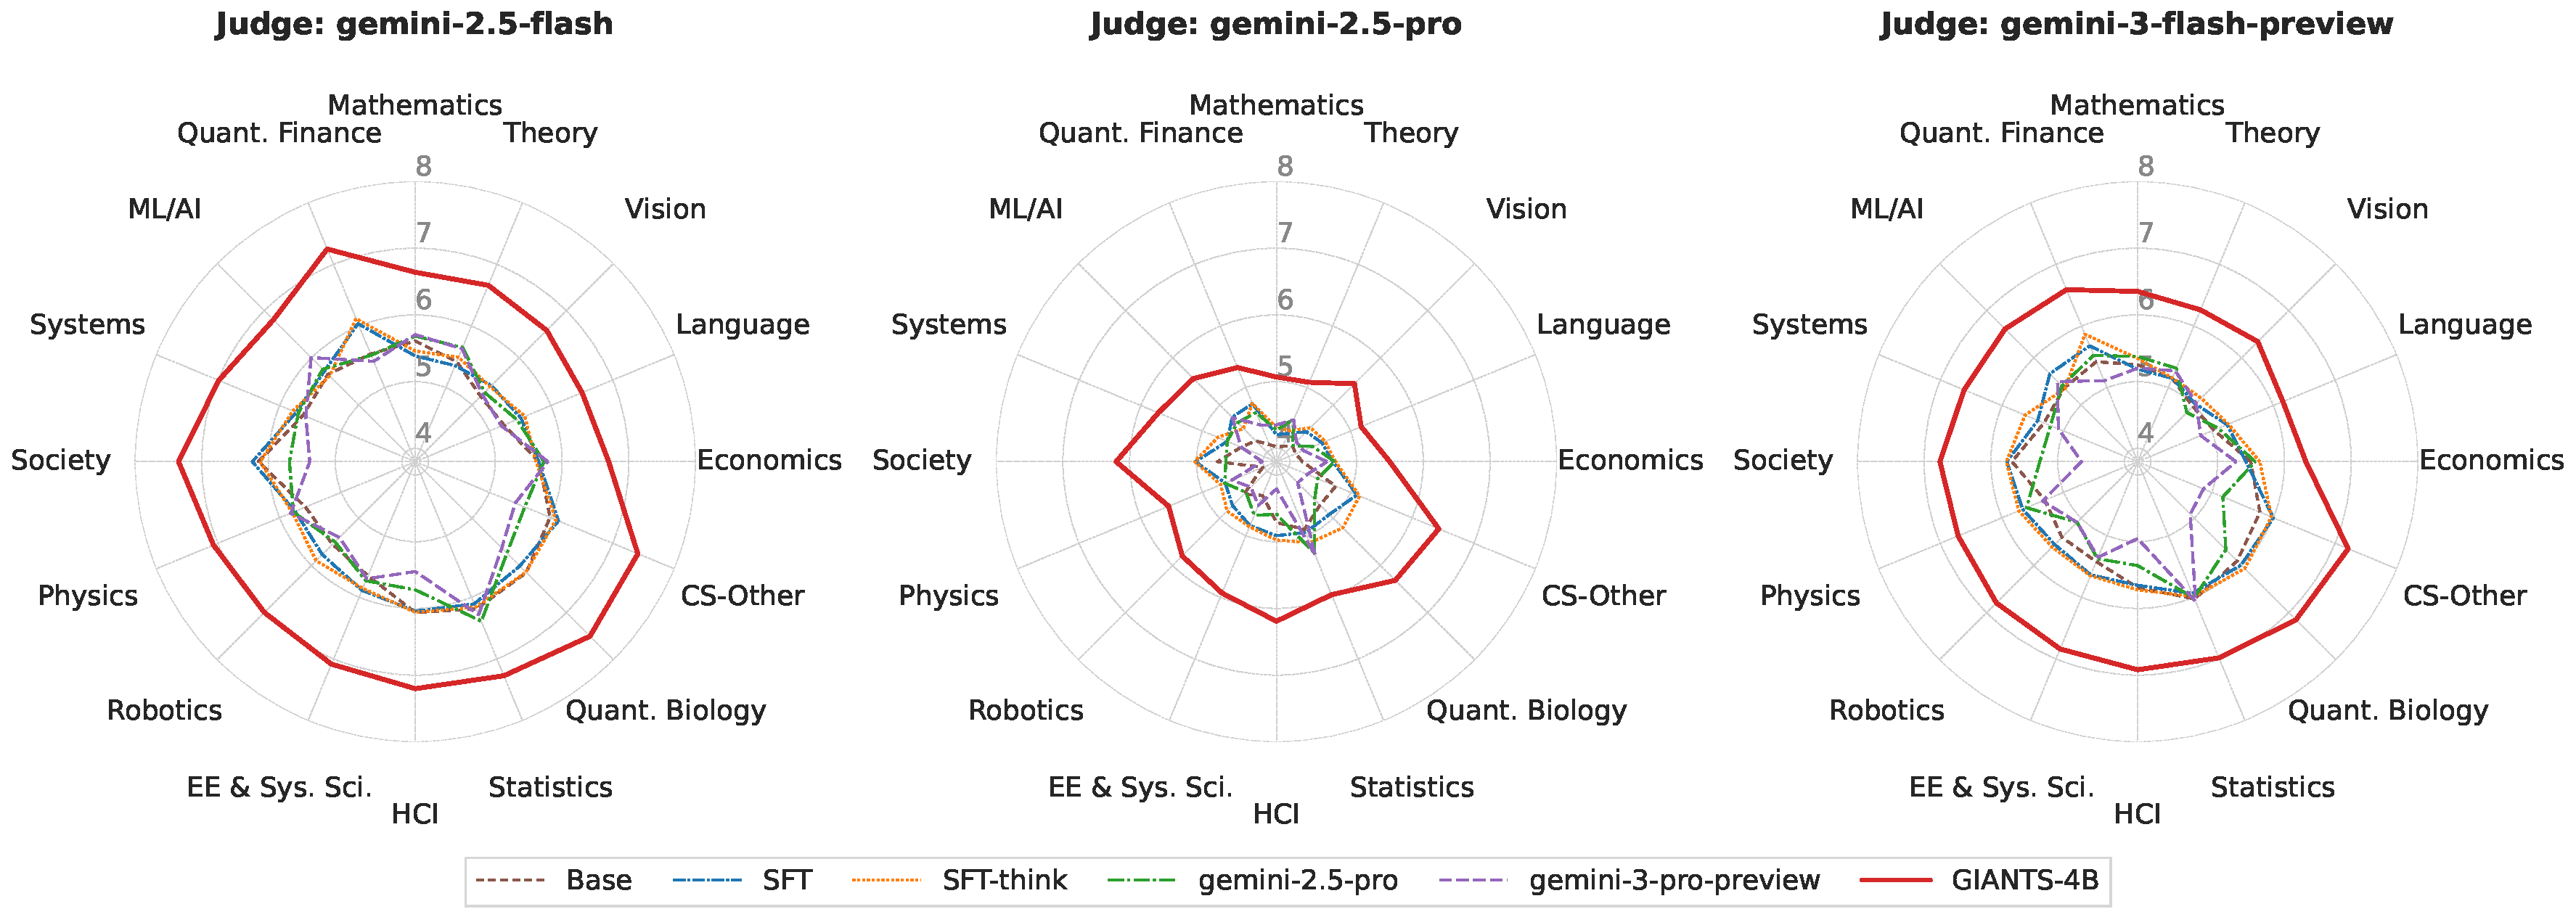
\includegraphics[width=\linewidth]{figs/all_domain_radar_3judges_unseen_parents.pdf}
    \vspace{-3mm}
    \caption{\textbf{Similarity scores on \emph{Test-unseen-parents}}. This is the subset of \ourbenchmark{} test set with only unseen parent papers.}
    \label{fig:all_domain_radar_3judges_unseen_parents}
\end{figure}


\section{Disclosure of LLM Use}
We used an LLM for light editing and revision of the manuscript, assistance with generating figures, and coding support throughout the project.

\section{More Human Eval Details}
\label{app:human_eval}

To validate the reliability of our automated metrics, we conducted a preliminary human evaluation study focusing on insight similarity. Annotators were tasked with scoring the semantic alignment between model-generated insights and ground-truth insights. To facilitate this process and ensure an unbiased environment, we developed a custom web interface, shown in Figure \ref{fig:placeholder}. Importantly, the human annotators were provided with the exact same scoring rubric and guidelines that were given to the LLM judge, allowing us to accurately measure the consistency between human judgment and our automated evaluation pipeline, with the exact context provided to the LLM judge.

\begin{figure}[H]
    \centering
    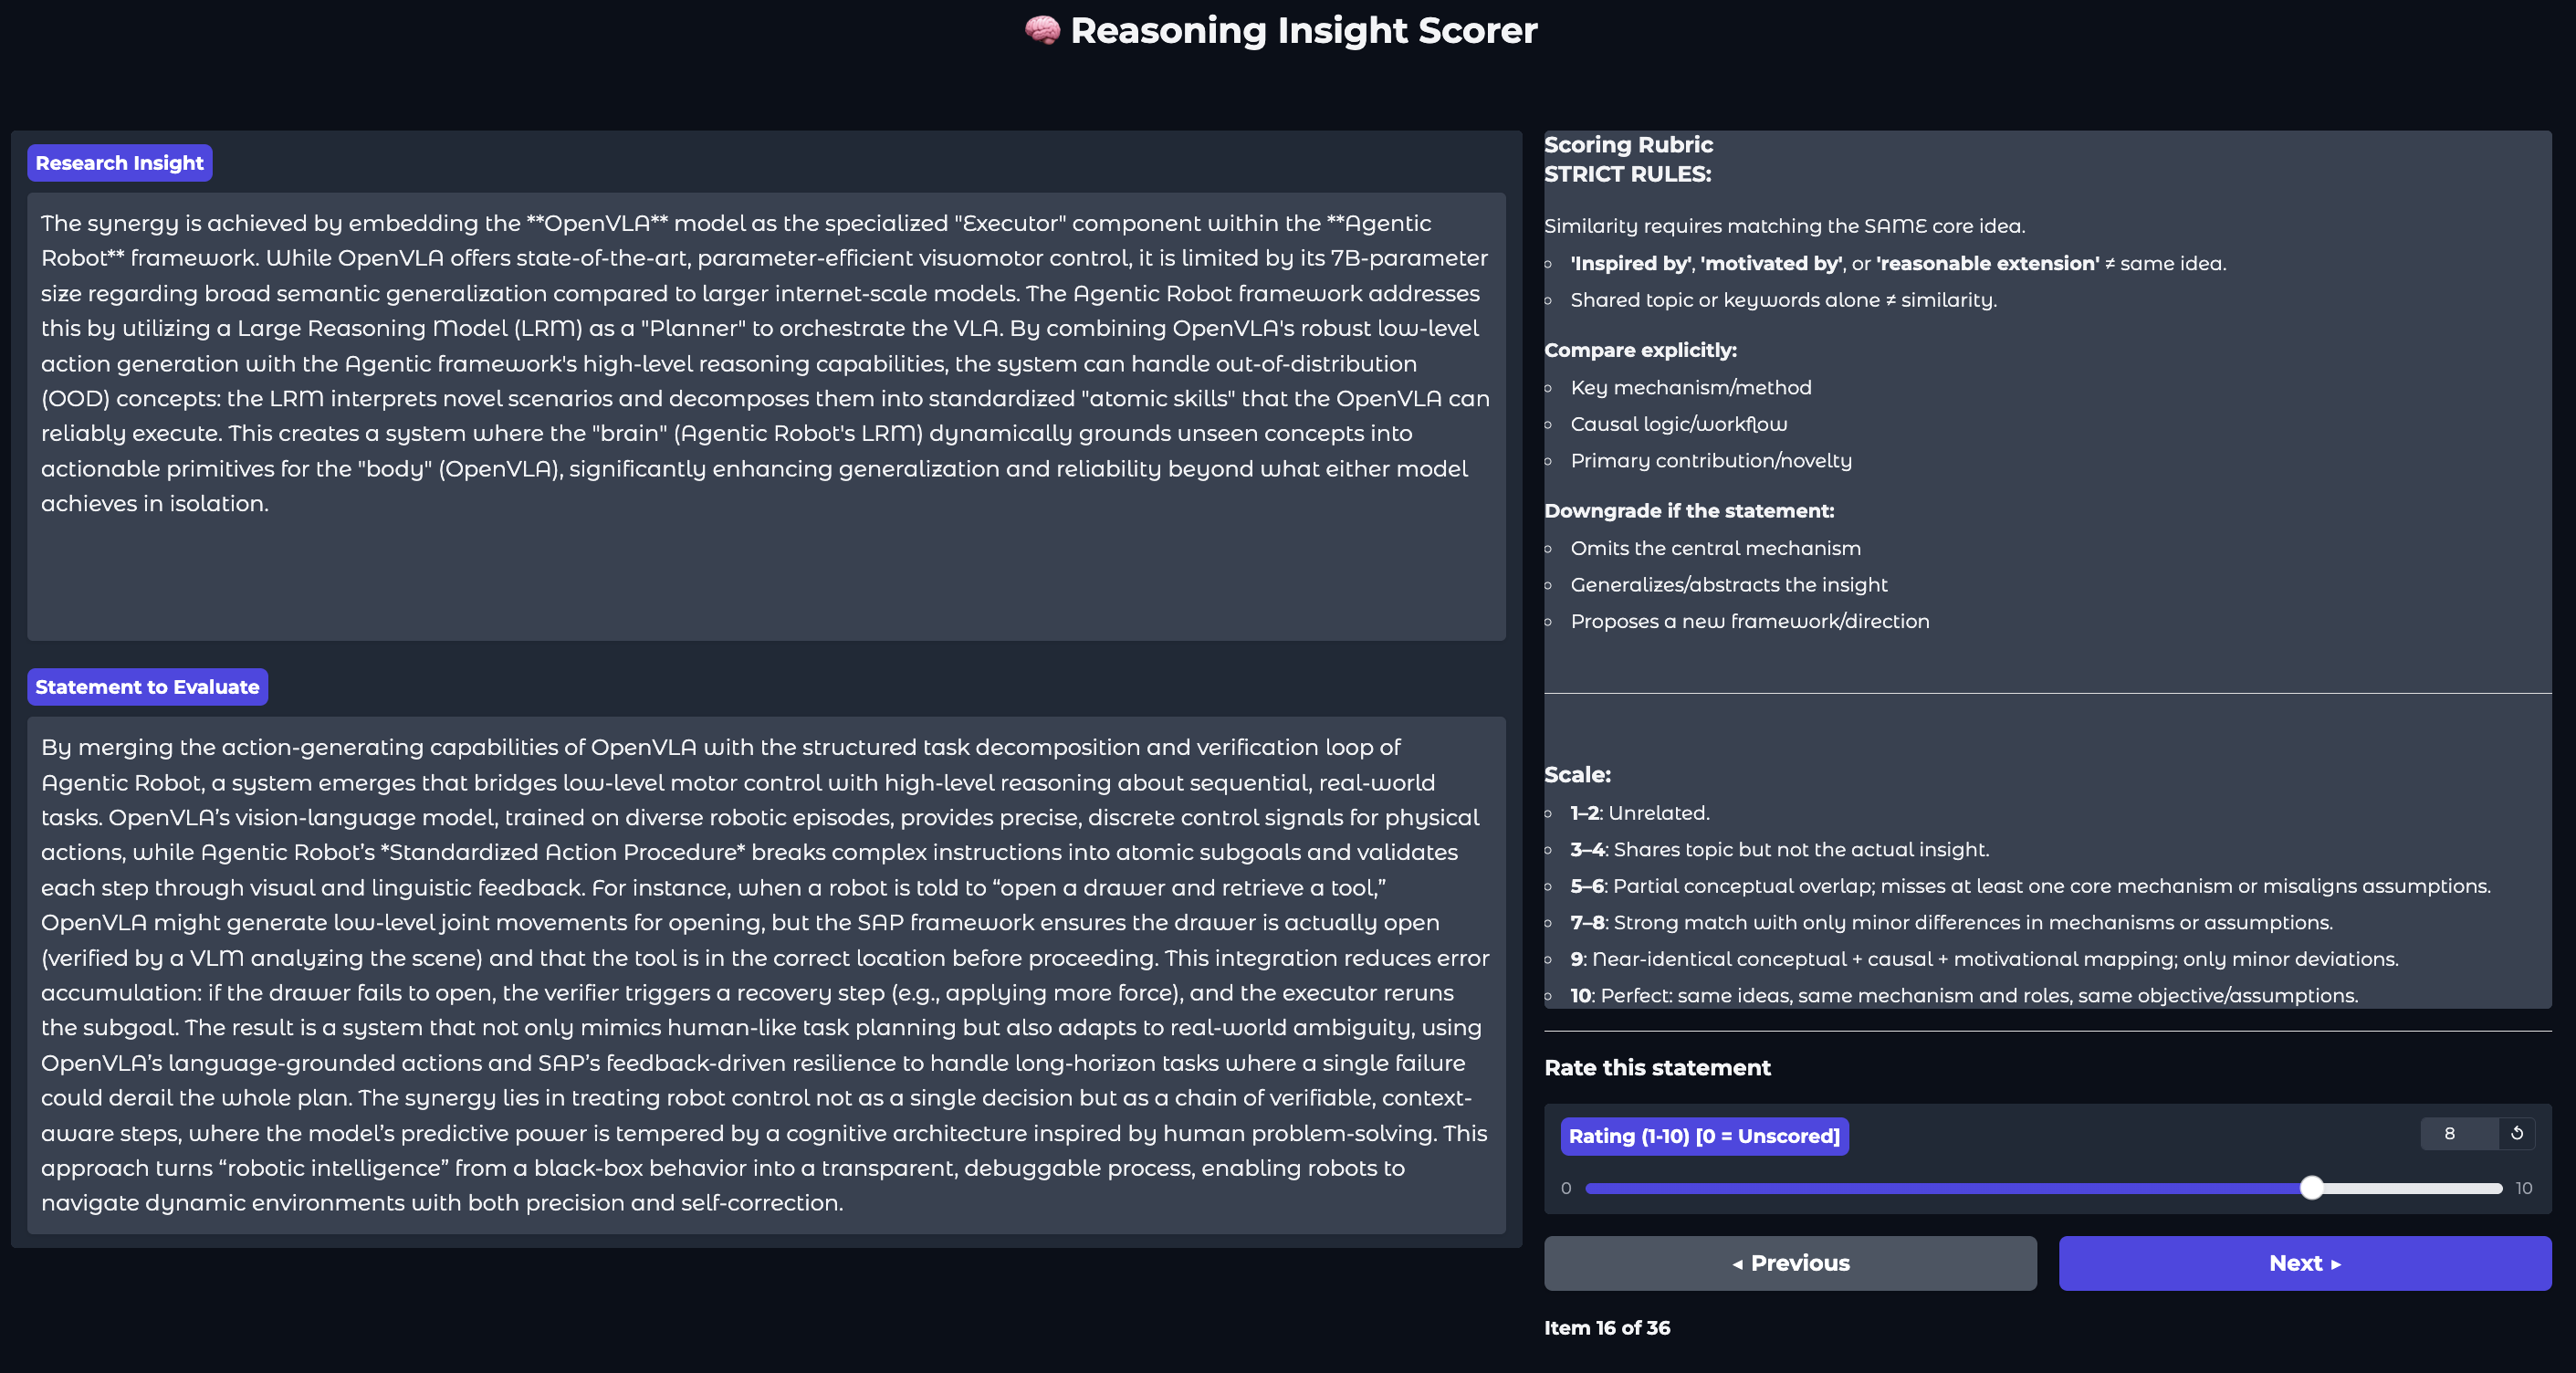
\includegraphics[width=0.8\linewidth]{figs/human_eval.png}
    \caption{\textbf{Human Eval Labeling App} Here is the Gradio interface that was used by human labelers to measure the consistency of LLM similarity with human ratings. The rubric provided to the humans exactly matched that provided to the LLM judge for consistency (with markdown formatting for human interpretability).}
    \label{fig:placeholder}
\end{figure}


\begin{figure}[H]
    \centering
    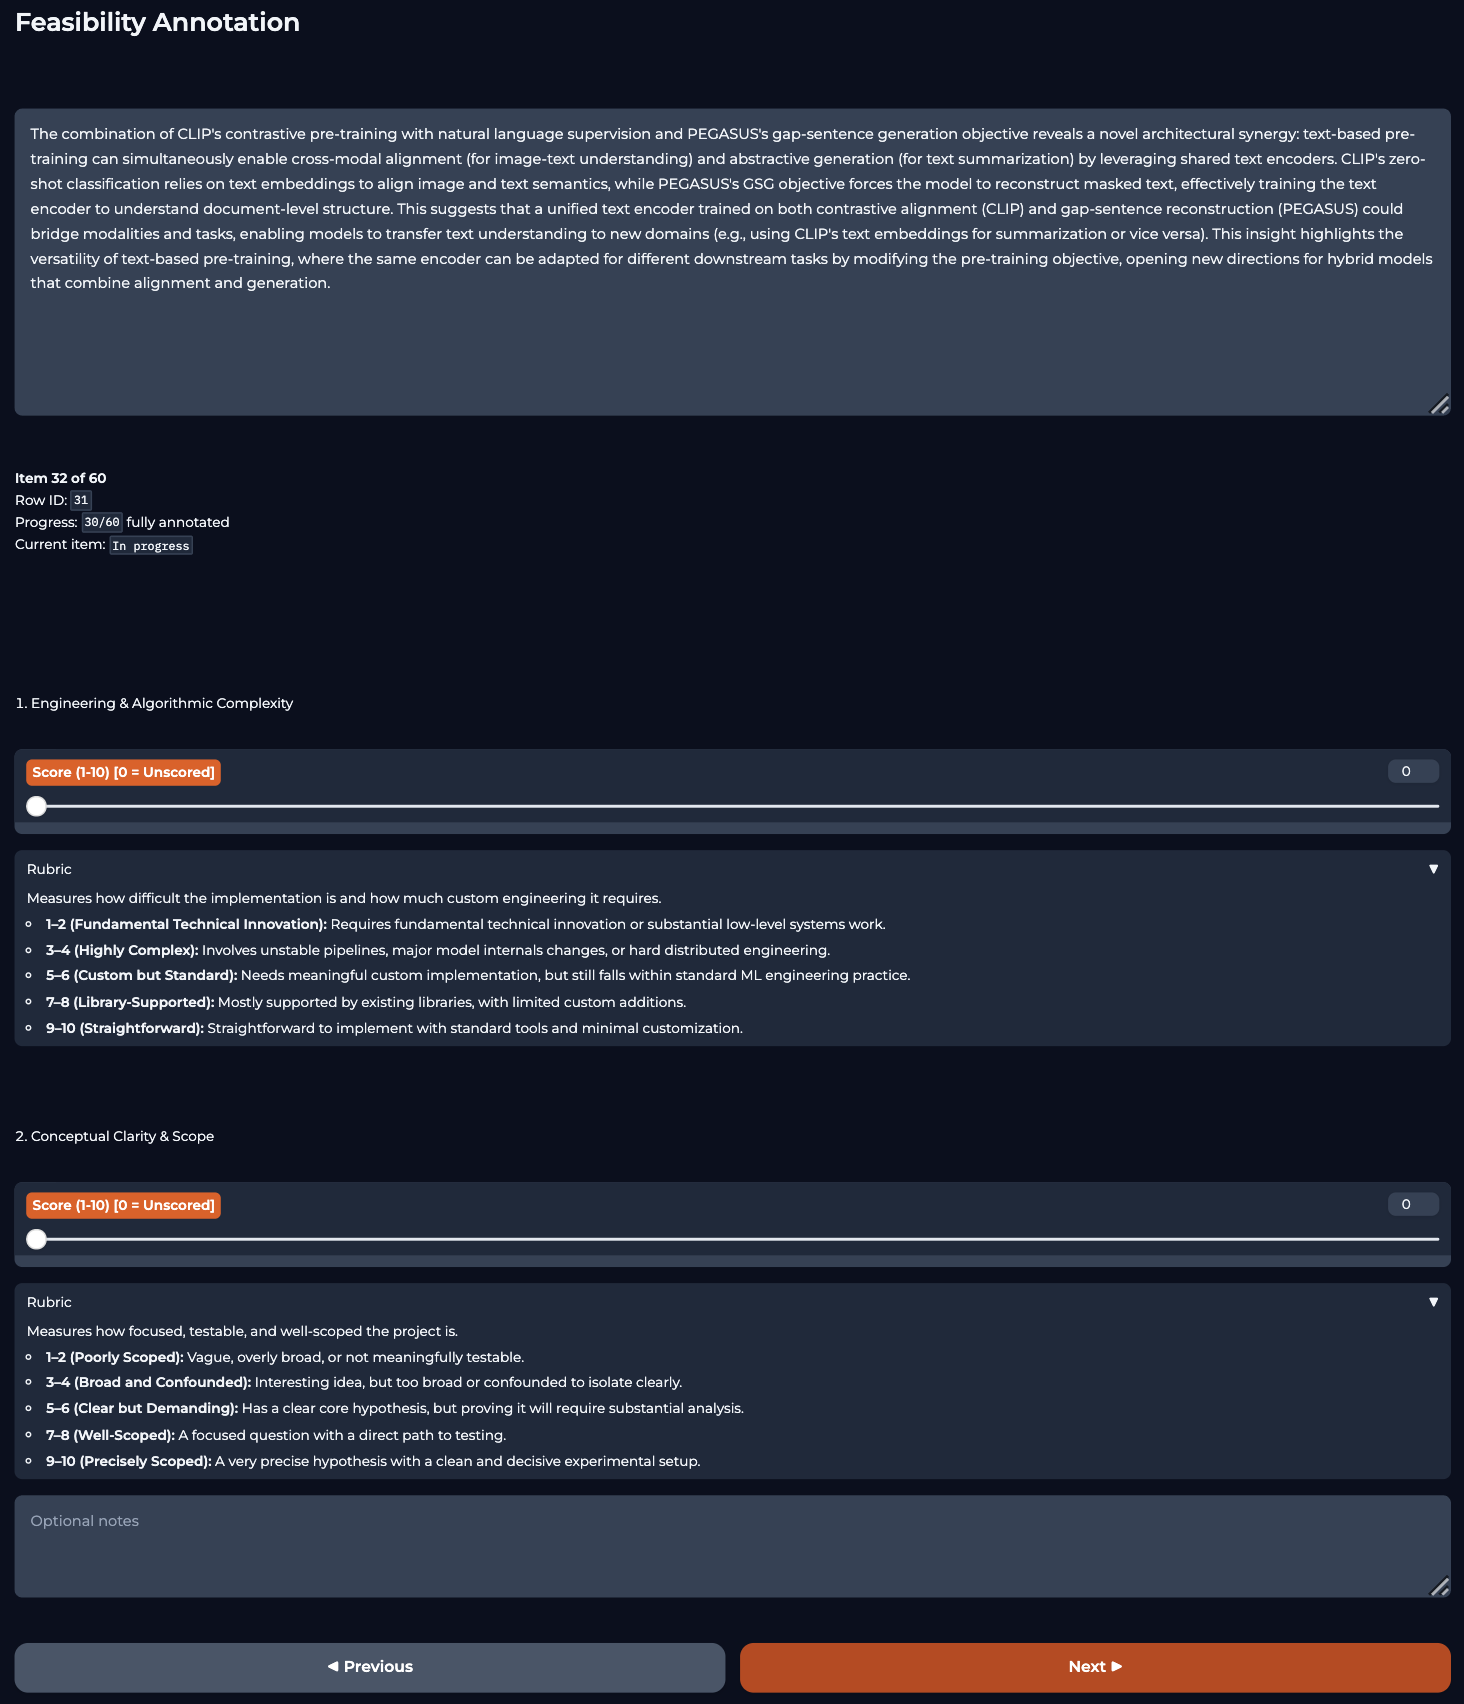
\includegraphics[width=0.8\linewidth]{figs/feasibility_human_eval.png}
    \caption{\textbf{Feasibility Human Eval Labeling App} Here is the Gradio interface that was used by human labelers to measure the feasibility of a research insight with human ratings. The rubric provided to the humans exactly matched that provided to the LLM judge for consistency (with markdown formatting for human interpretability).}
    \label{fig:placeholder}
\end{figure}




\end{document}
